
\documentclass[9pt, aspectratio=169]{beamer}

%
\usepackage{soul}
\usepackage{natbib}
\usepackage{hyperref}
\usepackage{bookmark}
\usepackage{graphicx}             
\graphicspath{{./Figuras/}}

\usepackage{makecell}
\usepackage[margin=1in]{geometry}
\usepackage{float}                
\usepackage{amsmath}
\usepackage{amscd}
\usepackage{amsfonts}
\usepackage{amssymb}
\usepackage{bbm}
\usepackage{booktabs}
\usepackage{nameref}
\usepackage{multirow}
\usepackage[nokeyprefix]{refstyle}
\usepackage{rotating}
\usepackage{threeparttable}
\usepackage{afterpage}
\usepackage{lscape}
\usepackage{enumerate}
\usepackage{caption}
\usepackage{subcaption}
\usepackage{epstopdf}
\usepackage{setspace}
\usepackage{svg}
\usepackage{dsfont}
\usepackage{amsthm}
\usepackage{tocloft}
\usepackage{etoc}
\usepackage{lmodern}
\usepackage{bm}

\epstopdfDeclareGraphicsRule{.tiff}{png}{.png}{convert #1 \OutputFile}
\AppendGraphicsExtensions{.tiff}

\epstopdfDeclareGraphicsRule{.tif}{png}{.png}{convert #1 \OutputFile}
\AppendGraphicsExtensions{.tif}

\usepackage{tikz}
\usetikzlibrary{shapes.geometric, arrows}
\usetikzlibrary{calc}
\usetikzlibrary{matrix}

\tikzset{ 
    table/.style={
        matrix of nodes,
        row sep=-\pgflinewidth,
        column sep=-\pgflinewidth,
        nodes={
            rectangle,
            draw=black,
            align=center
        },
        minimum height=1.5em,
        text depth=0.5ex,
        text height=2ex,
        nodes in empty cells,
%%
        every even row/.style={
            nodes={fill=gray!20}
        },
        column 1/.style={
            nodes={text width=2em,font=\bfseries}
        },
        row 1/.style={
            nodes={
                fill=black,
                text=white,
                font=\bfseries
            }
        }
    }
}


\usepackage{colortbl}

\newtheorem{theorem}{Theorem}
\newtheorem{claim}[theorem]{Claim}
\newtheorem{prop}[theorem]{Proposition} 
\newtheorem{cor}[theorem]{Corollary} 

\DeclareRobustCommand{\hlgr}[1]{{\sethlcolor{green}\hl{#1}}}


\usepackage{comment}
%para esconder columnas en tablas (enrique)
\usepackage{array}
\newcolumntype{H}{>{\setbox0=\hbox\bgroup}c<{\egroup}@{}}
\linespread{1.25}

\newcommand{\wh}{\widehat}
\usepackage{anyfontsize}

\usepackage[linesnumbered,vlined,ruled,commentsnumbered]{algorithm2e}

\DontPrintSemicolon
\newcommand{\To}{\mbox{\upshape\bfseries to}}
\usetheme[numbering=fraction, sectionpage=none,titleformat=smallcaps]{metropolis}


%\useoutertheme{smoothbars}
%\setbeamercolor{mini frame}{fg=white, bg=black}
%\setbeamercolor{section in head/foot}{fg=white, bg=black}

% !TEX TS-program = pdflatex
% !TEX encoding = UTF-8 Unicode


%%%%%%%%%%%%%%%%%%%%%%%%
% Usual LaTeX Packages %
%%%%%%%%%%%%%%%%%%%%%%%%

\usepackage{bbm}  %enrique agrwego 9/23/2023
\usepackage{unicode-math} %enrique agrwego 9/23/2023

\usepackage{pdfpages}
\usepackage{amsmath}
\usepackage{amsfonts}
\usepackage{amssymb}
\usepackage{graphicx}
\usepackage{mathrsfs} 			% For Weinberg-esque letters
\usepackage{cancel}				% For "SUSY-breaking" symbol
\usepackage{slashed}            % for slashed characters in math mode
\usepackage{bbm}                % for \mathbbm{1} (unit matrix)
\usepackage{amsthm}				% For theorem environment
\usepackage{multirow}			% For multi row cells in table
\usepackage{arydshln} 			% For dashed lines in arrays and tables
\usepackage{multirow}
\usepackage{multicol}
\usepackage{bigstrut}
\usepackage{setspace}
\usepackage{endnotes}
\usepackage{etex}
\usepackage{lmodern}
\usepackage{booktabs}
\usepackage{graphics}
\usepackage[flushleft]{threeparttable}
%\usepackage{enumitem}
%\setlist[itemize]{itemsep=2mm}
\usepackage{array}
\usepackage{color}
\usepackage{colortbl}
\usepackage{hyperref}
\usepackage{ifplatform}
\usepackage{dcolumn}
\usepackage{threeparttable}
 \usepackage{hyperref}
\usepackage{subcaption}
\usepackage{graphicx}

% Added by Roberto for table font size and appendix table of contents
\usepackage{etoolbox}
%\AtBeginEnvironment{table}{\scriptsize}
% -------------------------------

\usepackage{xcolor,sectsty}
\usepackage[many]{tcolorbox}

\definecolor{astral}{RGB}{46,116,181}

\captionsetup[subfigure]{justification=centering}

%% FONT
\usepackage[default,osfigures,scale=0.95]{opensans} %% Alternatively
%% use the option 'defaultsans' instead of 'default' to replace the
%% sans serif font only.

% TO SHOW NOTES ON ANOTHER SCREEN
%\usepackage{pgfpages}
%\setbeameroption{hide notes}
%\setbeameroption{show notes on second screen=right}
%FONT PACKAGE ==============================================
\usepackage[utf8]{inputenc}
\usepackage[T1]{fontenc}
\usepackage{appendixnumberbeamer}

% Doing Better Math
\usefonttheme{professionalfonts} % required for mathspec

%\captionsetup[subfigure]{justification=centering}
\usepackage[default,osfigures,scale=0.95]{opensans}
% HYPERREF =========================================================
% HyperRef Set up
\hypersetup{colorlinks=true,
           linkcolor=brown,
           bookmarks=true,
           anchorcolor=green,
           menucolor=cyan,
           citecolor=.,
           urlcolor=cyan,
           final=true
           }


% Code for Hiding Columns in Tables
\newcolumntype{H}{>{\setbox0=\hbox\bgroup}c<{\egroup}@{}}


\graphicspath{{images/}}	% Put all images in this directory. Avoids clutter.



% SOME COMMANDS THAT I FIND HANDY
% \renewcommand{\tilde}{\widetilde} % dinky tildes look silly, doesn't work with fontspec
\newcommand{\comment}[1]{\textcolor{comment}{\footnotesize{#1}\normalsize}} % comment mild
\newcommand{\Comment}[1]{\textcolor{Comment}{\footnotesize{#1}\normalsize}} % comment bold
\newcommand{\COMMENT}[1]{\textcolor{COMMENT}{\footnotesize{#1}\normalsize}} % comment crazy bold
\newcommand{\Alert}[1]{\textcolor{Alert}{#1}} % louder alert
\newcommand{\ALERT}[1]{\textcolor{ALERT}{#1}} % loudest alert
\newcommand{\red}{\textcolor[rgb]{1,0,0}}
\renewcommand\appendixname{Appendix}
\setbeamerfont{frametitle}{size=\large}


% BIBLIOGRAPHY (OPTION: BIBLATEX) ===========================================
\usepackage{csquotes}
\usepackage[natbib = true, backend = biber, style  = authoryear-icomp]{biblatex}
\addbibresource{References2.bib}
%\addbibresource{References.bib}
\addbibresource{library.bib}

\renewcommand{\cite}{\citet}
\ifmacosx
% UNCOMMENT IF COMPILING ON A MAC (No Fix in Linux but to install
% Biblatex 3.6)
% Problem with Commas in Biblatex
% http://tinyurl.com/yclhtz6s
\DeclareDelimFormat[cbx@textcite]{nameyeardelim}{\addspace}
% Redefine \cite to be \citet so that the silly bracket problem does
% not arise when using biblatex.
\fi


%%% HUGE KLUDGE JUST TO MAKE THE COMMA DISAPPEAR WHEN CITING PAPERS
%%% (BIBLATEX PROBLEM ONLY). COMMENT OUT WHEN COMPILING ON THE MAC
%%% WHICH DOESNT SEEM TO NEED THIS.
% \iflinux

% \makeatletter 
% \renewbibmacro*{textcite}{% 
%   \iffieldequals{namehash}{\cbx@lasthash} 
%     {\iffieldundef{shorthand} 
%        {\ifthenelse{\iffieldequals{labelyear}{\cbx@lastyear}\AND 
%                     \(\value{multicitecount}=0\OR\iffieldundef{postnote}\)} 
%           {\setunit{\addcomma}% 
%            \usebibmacro{cite:extrayear}} 
%           {\setunit{\compcitedelim}% 
%            \usebibmacro{cite:labelyear+extrayear}% 
%            \savefield{labelyear}{\cbx@lastyear}}} 
%        {\setunit{\compcitedelim}% 
%         \usebibmacro{cite:shorthand}% 
%         \global\undef\cbx@lastyear}} 
%     {\ifnameundef{labelname} 
%        {\iffieldundef{shorthand} 
%           {\usebibmacro{cite:label}% 
%            \setunit{% 
%              \global\booltrue{cbx:parens}% 
%              \addspace\bibopenparen}% 
%            \ifnumequal{\value{citecount}}{1} 
%              {\usebibmacro{prenote}} 
%              {}% 
%            \usebibmacro{cite:labelyear+extrayear}} 
%           {\usebibmacro{cite:shorthand}}} 
%        {\printnames{labelname}% 
%         \setunit{% 
%           \global\booltrue{cbx:parens}% 
%           \addspace\bibopenparen}% 
%         \ifnumequal{\value{citecount}}{1} 
%           {\usebibmacro{prenote}} 
%           {}% 
%         \iffieldundef{shorthand} 
%           {\iffieldundef{labelyear} 
%              {\usebibmacro{cite:label}} 
%              {\usebibmacro{cite:labelyear+extrayear}}% 
%            \savefield{labelyear}{\cbx@lastyear}} 
%           {\usebibmacro{cite:shorthand}% 
%            \global\undef\cbx@lastyear}}% 
%      \stepcounter{textcitecount}% 
%      \savefield{namehash}{\cbx@lasthash}}% 
%   \setunit{% 
%     \ifbool{cbx:parens} 
%       {\bibcloseparen\global\boolfalse{cbx:parens}} 
%       {}% 
%     \textcitedelim}} 
% \makeatother
% \fi
% ;



% BIBLIOGRAPHY (OPTION: BIBTEX) ===========================================
%\usepackage[elide]{natbib}
%\usepackage{bibentry}

% TITLE PAGE =============================================
\setbeamertemplate{title page}[default]
\setbeamercolor{titlelike}{parent=frametitle,fg=crimsonred}
\setbeamercolor{author}{fg=black,bg=white}
\setbeamercolor{institute}{fg=black,bg=white}
\setbeamercolor{date}{fg=black,bg=white}


% FRAME TITLE ==============================================
\setbeamercolor{background canvas}{bg=white}
\setbeamercolor{normal text}{fg=black}
\setbeamercolor{frametitle}{bg=white,fg=crimsonred}
\setbeamerfont*{frametitle}{series=\bfseries,size=\Large}

% BULLETPOINTS =========================================
\setbeamertemplate{itemize item}{\small\raise.2ex\hbox{\donotcoloroutermaths$-$}}
\setbeamertemplate{itemize subitem}{\small\raise.1ex\hbox{\donotcoloroutermaths$\circ$}}
\setbeamertemplate{itemize subsubitem}{\scriptsize\raise.1ex\hbox{\donotcoloroutermaths$\bullet$}}
\setbeamercolor{itemize item}{fg=lightash}
\setbeamercolor{itemize subitem}{fg=ash}
\setbeamercolor{itemize subsubitem}{fg=ash}
\setbeamercolor{enumerate item}{fg=ash}
\setbeamertemplate{enumerate item}{(\arabic{enumi})}
\setbeamercolor{enumerate subitem}{fg=ash}

% TABLE OF CONTENTS ========================================
\setbeamertemplate{section in toc}{\hypersetup{linkcolor=.}\Huge{\alert{\textbf{\colorbox{crimsonred}{\textcolor{white}{\inserttocsectionnumber}}\enskip\textcolor{crimsonred}{\inserttocsection}}}}}
\setbeamertemplate{section in toc shaded}{\hypersetup{linkcolor=.}\colorbox{lightgrey}{\textcolor{white}{\inserttocsectionnumber}}\enskip\inserttocsection}
\setbeamercolor{section in toc shaded}{fg=lightgrey}
%\setbeamertemplate{section in toc shaded}[default][50]

% NAVIGATION BAR ===============================================
\setbeamertemplate{headline}{%
\hypersetup{linkcolor=white}
\begin{beamercolorbox}[colsep=1.5pt]{upper separation line head}
\end{beamercolorbox}
\begin{beamercolorbox}{section in head/foot}
    \vskip2pt\insertsectionnavigationhorizontal{\paperwidth}{\hskip0pt plus1fill}{\hskip0pt plus1fill}\vskip2pt
\end{beamercolorbox}%
%\begin{beamercolorbox}[ht=10pt]{subsection in head/foot}%
%    \vskip2pt\insertsubsectionnavigationhorizontal{\paperwidth}{}{\hskip0pt plus1filll}\vskip2pt
%\end{beamercolorbox}%
\begin{beamercolorbox}[colsep=1.5pt]{lower separation line head}
\end{beamercolorbox}
}
\setbeamercolor{section in head/foot}{fg=white, bg=black}
\setbeamercolor{section in head/foot}{bg=ash}




% COLOR DEFINITIONS ==============================================
\definecolor{bbva}{RGB}{0,76,147}		% Neurtal red, good for dark or light bg
\definecolor{crimsonred}{RGB}{153,0,0}		% Neurtal red, good for dark or light bg
\definecolor{darkcrimsonred}{RGB}{105,0,0}	
\definecolor{darkcharcoal}{RGB}{25,25,25}		% Darker gray
\definecolor{charcoal}{RGB}{51,51,51}		% Darker gray
\definecolor{ash}{RGB}{100,100,100}			% medium gray
\definecolor{paleblue}{RGB}{0,102,102}		% More of an `ocean' color
\definecolor{turtlegreen}{RGB}{230,124,0}	% A more neutral green
\definecolor{paleale}{RGB}{204,204,102}		% Only for dark BG
\definecolor{lager}{RGB}{140,110,10}		% Use instead of pale ale for white BG
\definecolor{regal}{RGB}{90,0,120}			% A more neutral purple
\definecolor{jeans}{RGB}{20,30,150}			% A more neutral blue
\definecolor{red}{RGB}{137,37,46}
\definecolor{charcoal}{RGB}{82,89,85}
\definecolor{ash}{RGB}{100,100,100}
\definecolor{lightash}{RGB}{140,140,140}
\definecolor{gold}{RGB}{160,129,51}
\definecolor{navy}{RGB}{15,62,86}
\definecolor{crimsonred}{RGB}{153,0,0}
\definecolor{lightgrey}{RGB}{218,218,218}

\definecolor{azu_timeline}{rgb}{.267,  .329,  .416}
\definecolor{ama_timeline}{rgb}{1,  .753,  0}
\definecolor{nar_timeline}{rgb}{ .776,  .349,  .067}
\definecolor{roj_timeline}{RGB}{189, 0, 13}
\definecolor{ver_timeline}{rgb}{.329,  .51,  .208}







%% FOOTLINE ====
\setbeamertemplate{footline}{%
  \begin{beamercolorbox}[sep=0.5em,wd=\paperwidth,leftskip=0.5em,rightskip=0.5em]{footlinecolor}
    %\includegraphics[scale=0.07,height=10pt]{images/image1.png}
  Pawn Loans \hfill%
    \tiny{\insertframenumber/\inserttotalframenumber}
    %\includegraphics[scale=0.25,height=10pt]{images/image2.png}
  \end{beamercolorbox}%
}
\setbeamercolor{footlinecolor}{fg=white,bg=ash}






%% Does a Progress Bar for the Talk at the Bottom of the Page
%% http://tex.stackexchange.com/questions/59742/progress-bar-for-latex-beamer

% \setbeamercolor{progress bar progress}{use=progress bar,bg=progress bar.fg}
% \defbeamertemplate{footline}{progress bar}{
%   \dimen0=\paperwidth
%   \multiply\dimen0 by \insertframenumber
%   \divide\dimen0 by \inserttotalframenumber
%   \edef\progressbarwidth{\the\dimen0}

%   \leavevmode%
%   \begin{beamercolorbox}[wd=\paperwidth,ht=1.75ex,dp=1ex]{progress
%       bar}
%     \begin{beamercolorbox}[wd=\progressbarwidth,ht=1.75ex,dp=1ex]{progress bar progress}
%     \end{beamercolorbox}%
%     \insertframenumber{} / \inserttotalframenumber
%   \end{beamercolorbox}%
% }
% \setbeamertemplate{footline}[progress bar]
% \setbeamercolor{progress bar}{fg=blue!50!black,bg=white!50!black}
% ;
%%%%%%%%%%%%%%%

%\usetikzlibrary{backgrounds}
%\usetikzlibrary{mindmap,trees}	% For mind map
% http://www.texample.net/tikz/examples/computer-science-mindmap/

%%% Local Variables:
%%% mode: latex
%%% TeX-master: t
%%% End:


% %%%% MAURICIO ADDED THESE
% \setbeamerfont{frametitle}{size=\large}
% \setbeamertemplate{navigation symbols}{}
% \newcolumntype{L}[1]{>{\raggedright\let\newline\\\arraybackslash\hspace{0pt}}m{#1}}
% \newcolumntype{C}[1]{>{\centering\let\newline\\\arraybackslash\hspace{0pt}}m{#1}}
% \newcolumntype{R}[1]{>{\raggedleft\let\newline\\\arraybackslash\hspace{0pt}}m{#1}}

% \def\zapcolorreset{\let\reset@color\relax\ignorespaces}
% \def\colorrows#1{\noalign{\aftergroup\zapcolorreset#1}\ignorespaces}

% \newcolumntype{H}{>{\setbox0=\hbox\bgroup}c<{\egroup}@{}}


% %center text in tables
% \newcommand{\specialCellCenter}[2][c]{\begin{tabular}[#1]{@{}c@{}}#2\end{tabular}}
% \newcommand{\specialcell}[2][l]{\begin{tabular}[#1]{@{}l@{}}#2\end{tabular}}
% \def\sym#1{\ifmmode^{#1}\else\(^{#1}\)\fi}
% \setbeamertemplate{note page}[compress]
% \setbeamerfont{note page}{size=\tiny}
% \setbeameroption{hide notes}
% \setbeamersize{text margin left=0.2in,text margin right=0.2in}
% \setbeamertemplate{footline}{}



%%%%% HACER HIGHLIGHT DE DIFERNETES PARTES

\usepackage[beamer,customcolors]{hf-tikz}
\usetikzlibrary{calc}
\tikzset{hl/.style={%
    set fill color=red!80!black!40,
    set border color=red!80!black,
  },
}
\RenewDocumentCommand{\tikzmarkin}{r<> o m D(){\belowrightoff} D(){\aboveleftoff}}{%
  \IfNoValueTF{#2}{%true-val
    \only<#1>{\tikz[remember picture,overlay]
      \draw[line width=1pt,rectangle,disable rounded corners,fill=\fcol,draw=\bcol]
      (pic cs:#3) ++(#4) rectangle (#5) node [anchor=base] (#3){}
      ;}%
  }{%false-val
    \only<#1>{\tikz[remember picture,overlay]
      \draw[line width=1pt,rectangle,disable rounded corners,fill=\fcol,draw=\bcol,#2]
      (pic cs:#3) ++(#4) rectangle (#5) node [anchor=base] (#3){}
      ;}}%
}

\newenvironment{transitionframe}{
  \setbeamercolor{background canvas}{bg=crimsonred!30}
  \begin{frame}}{
    \end{frame}
}

\newcommand{\transitiontext}[1]{\begin{center} \Huge{\textcolor{crimsonred}{#1}}\end{center}}

%%% MAX





\title{Structured Payments in Pawnshop Borrowing:\\
Mandates vs. Choice}
\author{Craig McIntosh\inst{1} \and Isaac Meza\inst{2} \and Joyce Sadka\inst{3} \and Enrique Seira\inst{4} \and Francis J. DiTraglia\inst{5} }
\institute[UTran]{\inst{1} UCSD, \inst{2} Harvard , \inst{3} ITAM , \inst{4} MSU , \inst{5} Oxford} 
                      
\date{April 2025}

%\setbeamercolor{section in head/foot}{bg=darkcrimsonred}
\setbeamersize{text margin left=11pt, text margin right=11pt}
%\setbeamertemplate{section in toc}[square]




%%%%%%%%%%%%%%%%%%%%%%%%%%%%%%%%%%%%%%%
%%%%%%%%%%%%%%%%%%%%%%%%%%%%%%%%%%%%%%

\begin{document}


\begin{frame}[c, noframenumbering]%{\phantom{title page}}
% The \phantom{title page} is a kludge to get the red bar on top
\titlepage
\end{frame}


\begin{frame}{Pawnshop loans: prevalent and understudied}

\begin{itemize}
     \item Pawn loans are small, short-term loans, typically used for emergencies.
    \begin{itemize}
        \item Used by borrowers who don't have much access to credit: no credit or income checks.
    \end{itemize}
    \vfill \item \textbf{Overcollateralized}. Those loans involve surrendering highly liquid collateral (gold), in return for an immediate loan of much smaller value.  
    \begin{itemize}
        \item Unlike mortgages, pawn lender retains the entire value of the collateral under default along with any payments.
        \item For a given loan, lenders earn more by default.
    \end{itemize}    
    \vfill \item Pawn lending is very prevalent in the world (Carter \& Skiba, 2012). 
    \begin{itemize}
        \item 11,000 pawn shops in US, with 30m clients and \$14b revenues; in China \$43b.
        \item Our partner lender: 1m clients in 3 yrs (2.3m microfinance clients in Mexico, Pedroza, 2010).
    \end{itemize}
\end{itemize}    

\end{frame}




\begin{frame}{Flexibility and high default}
    \begin{itemize}
    \item Pawn loans are highly \textbf{flexible:} pay-when-you-want within 90 days, no structured payments, no reminders.
        \begin{itemize}
            \item This lack of structure contrasts with microfinance loans.
        \end{itemize}
    \vfill \item High default rates, 44\% in our data (an order of magnitude larger than microfinance).
    \begin{itemize}
        \item Subjective value higher than gold value $\Rightarrow$ inefficient to lose.
        \item Gold-buying stores (avg of 2.8) close to pawn shops (pay $\approx$ 100\% of its gold value).
    \end{itemize}
     \item \vfill \textbf{Optimistic borrowers}: In our data, borrowers are very optimistic about recovery: avg. subjective probability of recovery (0-100) in our data is 92\%, and 72\% say recovery is certain.
     \begin{itemize}
         \item Conditional on default: more than 2/5 pay towards recovery (avg. 42\% loan value).
     \end{itemize}
\end{itemize}
\end{frame}




\begin{frame}{Questions}
     \begin{enumerate}
         \item  Could borrowers benefit from \textbf{structured} (frequent) payments, but contract not be offered by lenders?
         \item \vfill If such a contract were offered, would it be demanded by borrowers?
        \item \vfill Would \textbf{mandating} frequent payments reduce financing costs more than giving a menu of \textbf{choices}?
        \item \vfill What is the treatment effect of structured payments on those who would \textbf{not} choose them (TuT)? 
        \begin{itemize}
            \item Are non choosers leaving money on the table?
        \end{itemize} 
     \end{enumerate}
\end{frame}



\begin{frame}{Outline}
     \large   
     \begin{itemize}
        \item \textbf{Context: Borrowers, contracts, data, outcomes}
         \item \vfill ``Mandates-Choice'' Experimental Design
         \vfill\item Main results
          \vfill\item Exploiting ``Mandates-Choice'' Design: ToT, TuT
         \vfill\item Why low demand (mostly speculative)
         %\vfill \item Targeting?
     \end{itemize}
\end{frame}



\begin{frame}{Context}
\vspace{-.4in}
\begin{columns}
\begin{column}{.45\textwidth}
\begin{figure}[H]
    \begin{center}
    \caption{Pawnshop}
        
\includegraphics[width=0.75\textwidth]{Figuras/empenio2_.png}
    \end{center}
    \end{figure}
\begin{figure}[H]
    \begin{center}
    \caption{Appraisers  inside a pawnshop}
        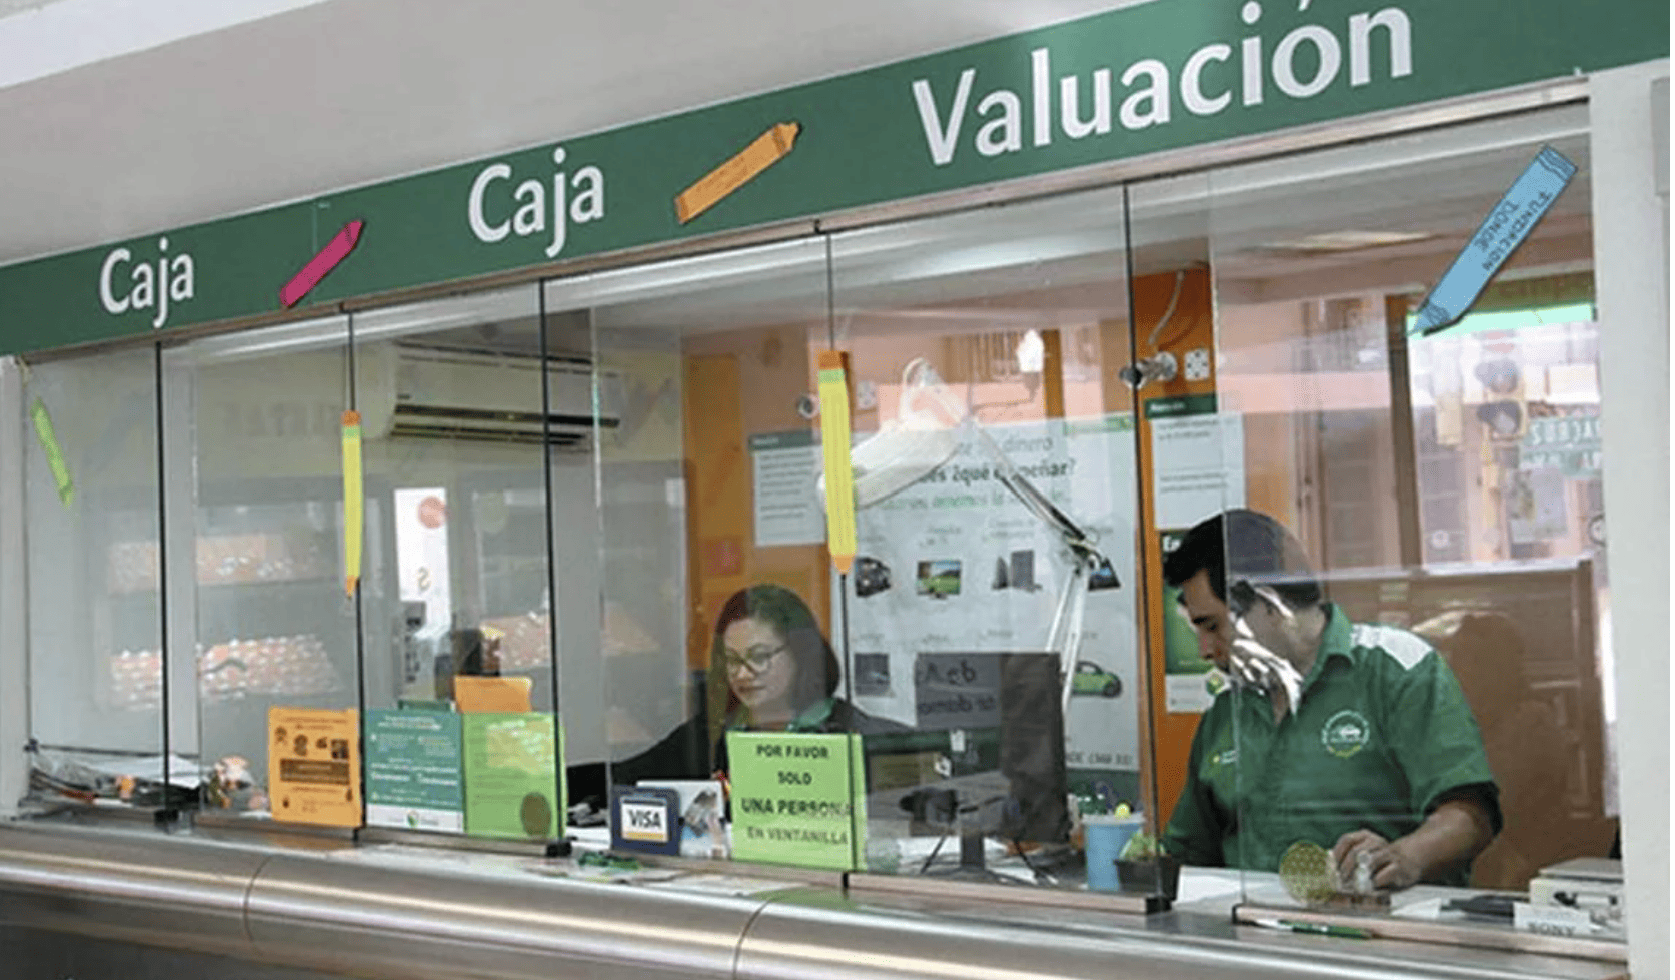
\includegraphics[width=0.7\textwidth]{Figuras/empenio9_.png}
    \end{center}
    \end{figure}    
    \end{column}
\begin{column}{.45\textwidth}
\begin{figure}[H]
    \begin{center}
    \caption{Waiting for appraisal}
        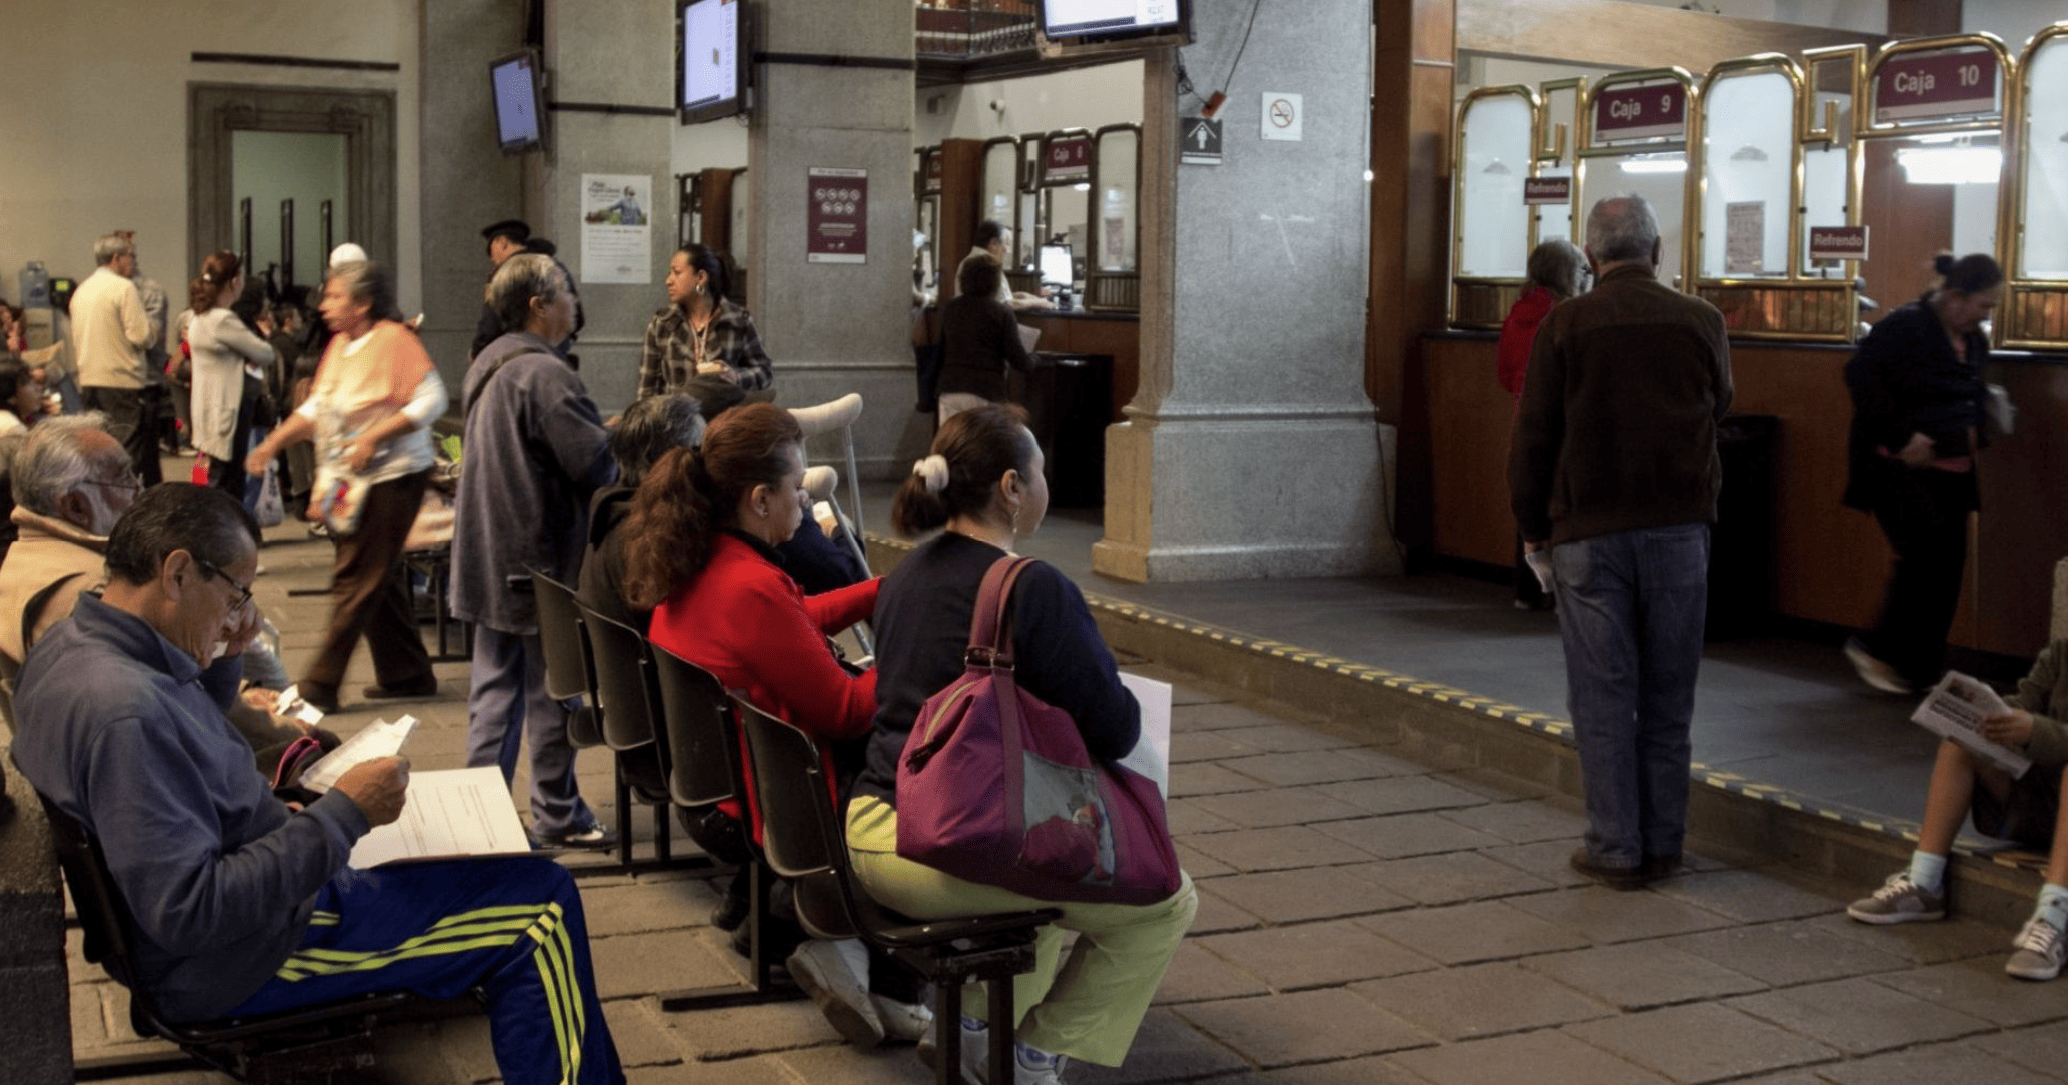
\includegraphics[width=0.7\textwidth]{Figuras/empenio11_.png}
    \end{center}
    \end{figure}
\begin{figure}[H]
    \begin{center}
    \caption{Lost pawns which are for sale}
        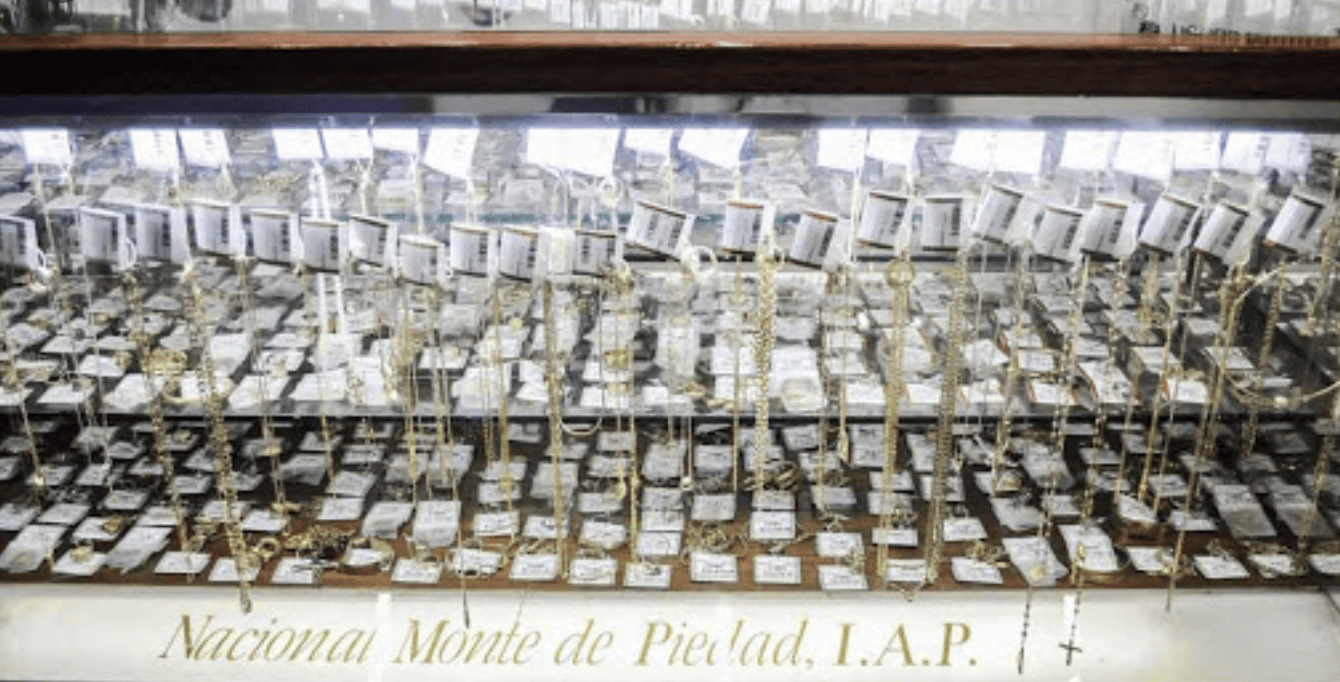
\includegraphics[width=0.75\textwidth]{Figuras/empenio3_.png}
    \end{center}
    \end{figure}    
    \end{column}    
    \end{columns}
\end{frame}



%%%%%%%%%%%%%%%%%%%%%%%%%%%%%%%%%%%%%%%%%

\section{Context}

\begin{frame}{Status quo contract (control group)}

\begin{itemize}
    \item Loan: 70\% of gold value in cash. Avg loan $\approx$ \$100USD.
    \item Loan term:  90 days.
    \item Repossession: if payments do not cover interest + capital, the lender sells the pawn at gold value.
    \item Interest rate: 7\% monthly rate on outstanding balances accumulated daily.
    \item No pre-payment penalties, no reminders.
    \item Borrowers can refinance the loan under the same terms if they pay incurred interest.
    \item Payments are first allocated to cover interest and lastly to capital.
    \item \alert{Pay when you want} before 90 days $\Leftarrow$ \pause We will impose ``Structured payments'' --- 3 equal-size payments per month.
\end{itemize}
    
\end{frame}




\begin{frame}{Data}
\begin{itemize}
    \item \textbf{Administrative data} 
    \begin{itemize}
        \item 1 month before, during, and 8 months after  experiment.
        \item Unique identifier for each client and each pawn.
        \item Value of the item, money loaned, date of pawning.
        \item For all payments: date,  amounts, and allocation to interest and capital.
        \item Fees incurred.
        \item Whether the client lost the pawn, recovered it, or refinanced the contract and when.
    \end{itemize} 

    \vfill \item \textbf{Survey data}
    \begin{itemize}
        \item During experiment, we asked clients to complete a 5-minute survey before going to the teller window to appraise their piece and before treatment status was known to them.
        \item Demographics, subjective probability of recovering, vulnerability, education, present-bias, experience pawning, cost of going to branch, the subjective value, etc.
        \item We use this data only in the last part to (a) estimate CATEs, (b) discuss some mechanisms.
    \end{itemize}
\end{itemize}    
\end{frame}




\begin{frame}{Main outcomes: financial cost and default}
\label{fc_outcome}
\begin{itemize}
    \item We are interested in measuring the financial cost of borrowing, which includes the cost of losing the pawn.
    \vfill \item We will measure loan default using an indicator $\mathds{1}(\text{Default}_i)$, and the cost in pesos using the following definition that capture borrower outlays:    
\end{itemize}

\vspace{-.1in}

\begin{equation*}
  \text{Financial Cost}_i =
  \begin{cases}
    \sum_t P^{I}_{it} + \sum_t P^{F}_{it}   & \text{if } \mathds{1}\text{(Default)}_i=0\\
     \sum_t P^{I}_{it} + \sum_t P^{F}_{it} + \sum_t P^{C}_{it} + (\text{Value}_i - \text{Loan}_i) & \text{if } \mathds{1}\text{(Default)}_i=1 
  \end{cases}
\end{equation*}

   % \begin{equation*}
   %  \text{Financial Cost}_i =  \underbrace{\sum_t P^i_{it}}_{\text{Pay to Interest}} + \underbrace{\sum_t P^f_{it}}_{\text{Pay to Fees}}  + \mathds{1}(\text{Default}_i) \times \left[(\text{Value}_i - \text{Loan}_i)+ \underbrace{\sum_t P^c_{it}}_{\text{Pay to Capital}} \right]
   % \end{equation*}

\vfill \begin{itemize}
    \item We also show results in APR-like ``effective'' yearly interest rate (norm. FC by loan value and term).
\end{itemize}

% \pause \vspace{.2in}
% \: \: \: \: APR: ``effective'' interest rate:
%    \begin{equation*}
%     (\text{APR})_i =\left( 1 + \frac{\frac{\text{Financial Cost}_i}{\text{Loan Value}_i}}{\text{loan term}_i}\right)^{\text{loan term}_i}-1 
% \end{equation*}

   \vspace{.1in}
\begin{itemize}
    \item We \alert{will not talk about welfare}, only financial cost.
    \begin{itemize}
        \item Welfare could depend on reduced liquidity, anxiety from monthly payments, etc.
        \item If you have ideas on how to do welfare let me know.
    \end{itemize}
\end{itemize}
\end{frame}




\begin{frame}{Outline}
     \large   
     \begin{itemize}
        \item Context: Borrowers, contracts, data, outcomes
         \item \vfill \textbf{``Mandates-Choice'' Experimental Design}
         \vfill\item Main results
          \vfill\item Exploiting ``Mandates-Choice'' Design: ToT, TuT
         \vfill\item Why low demand
         
     \end{itemize}
\end{frame}



%%%%%%%%%%%%%%%%%%%%%%%%%%%%%%%%%%%%%%%%%%%%%%%%%

\section{M-C design}



\begin{frame}{Mandates-Choice Design}
\label{treatment_arms}
   \begin{itemize}
    \vfill \item Randomization at the branch-day level.  Analysis at the pawn level.
    \begin{enumerate}
        \vfill \item Status quo contract (Control, 1770 obs)
       \vfill \item Structured payments (Frequent payments, 1954 obs)
       \vfill \item Choice between the two (2580 obs)
    \end{enumerate}
       \vfill \item  This design enables us to explore whether giving Choice saves borrowers more money than assigning them to a Structured payment contract or Status-quo.
       \vfill \item The existence of a Choice arm allows us to measure if there is demand for such a contract. Will also allow more cool stuff... 
\end{itemize}
\end{frame}



\begin{frame}{More details on implementation}
    \begin{itemize}
        \item Randomization built into IT system
        \item No person knew sequence of days-contract type.
        \item  Personnel were told that consecutive same contract-type could occur, and that randomization was happening in many branches.
        \item We had materials to explain the contract in simple terms.
        \item Borrowers explained back the contract.
        \item Appraisers no incentive either way (paid flat wage). Enumerators were there every day all day.
        \item Virtually no borrower left the branch without pawning.
        \item They seem to like this lender: 87\% pawned there before.
        \item Stick to branch: we cannot find experimental subjects in 2 different experimental branches. 
    \end{itemize}
\end{frame}




\begin{frame}{Standard (status quo) contract}
\vspace{-.2in}
    \begin{figure}[H]
    \label{ExplanatoryMaterial1}
    \begin{center}
        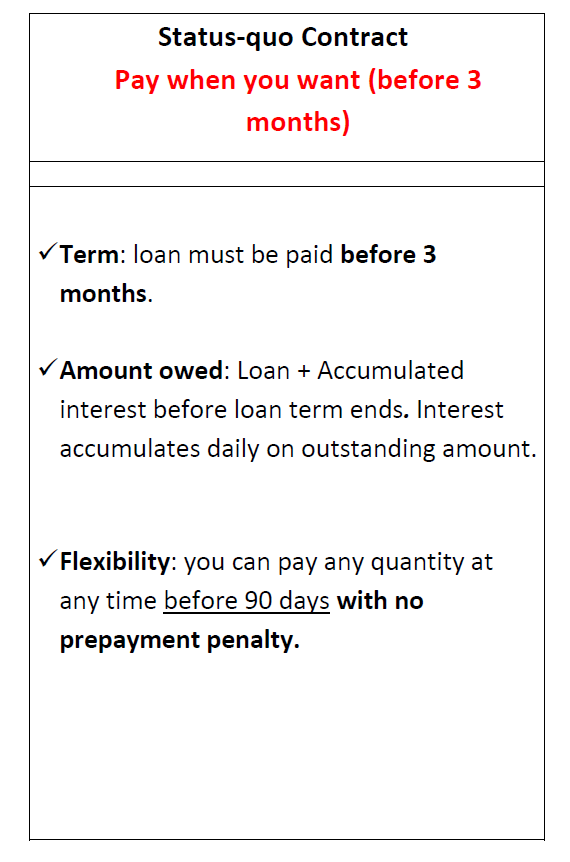
\includegraphics[width=0.34\textwidth]{Figuras/sq_contract.png}
    \end{center}
\end{figure}
\end{frame}



\begin{frame}{Structured payments contract}
%\vspace{-.1in}
\begin{columns}
\begin{column}{.45\textwidth}
   \begin{itemize}
       \vfill \item New contract identical to the status quo contract, except that it enhances the regularity of payments.
       \vspace{.2in}
       \vfill \item Penalty fee not large < 1 USD on avg loan; $\approx$avg. transport cost to go to branch.
       \vspace{.2in}
       \vfill \item We view it as a way to increase salience of monthly payment.
    \end{itemize}
    \end{column}
\begin{column}{.45\textwidth}
    \vspace{-.3in}
        \begin{figure}[H]
            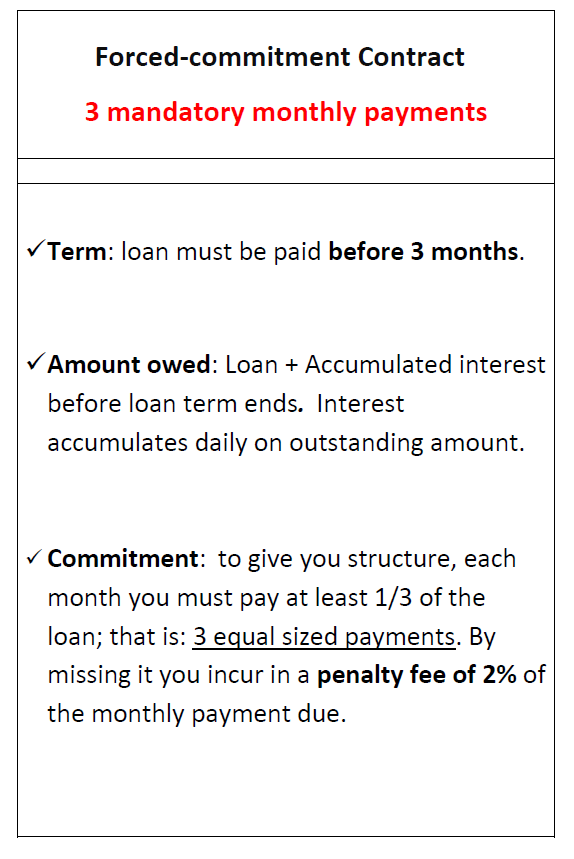
\includegraphics[width=0.78\textwidth]{Figuras/fc_contract.png}
        \end{figure}
    \end{column}
    \end{columns}
\end{frame}



 \begin{frame}{Timeline and sample size}
\vspace{-.3in}
 \begin{figure}[H]
 \begin{center}
         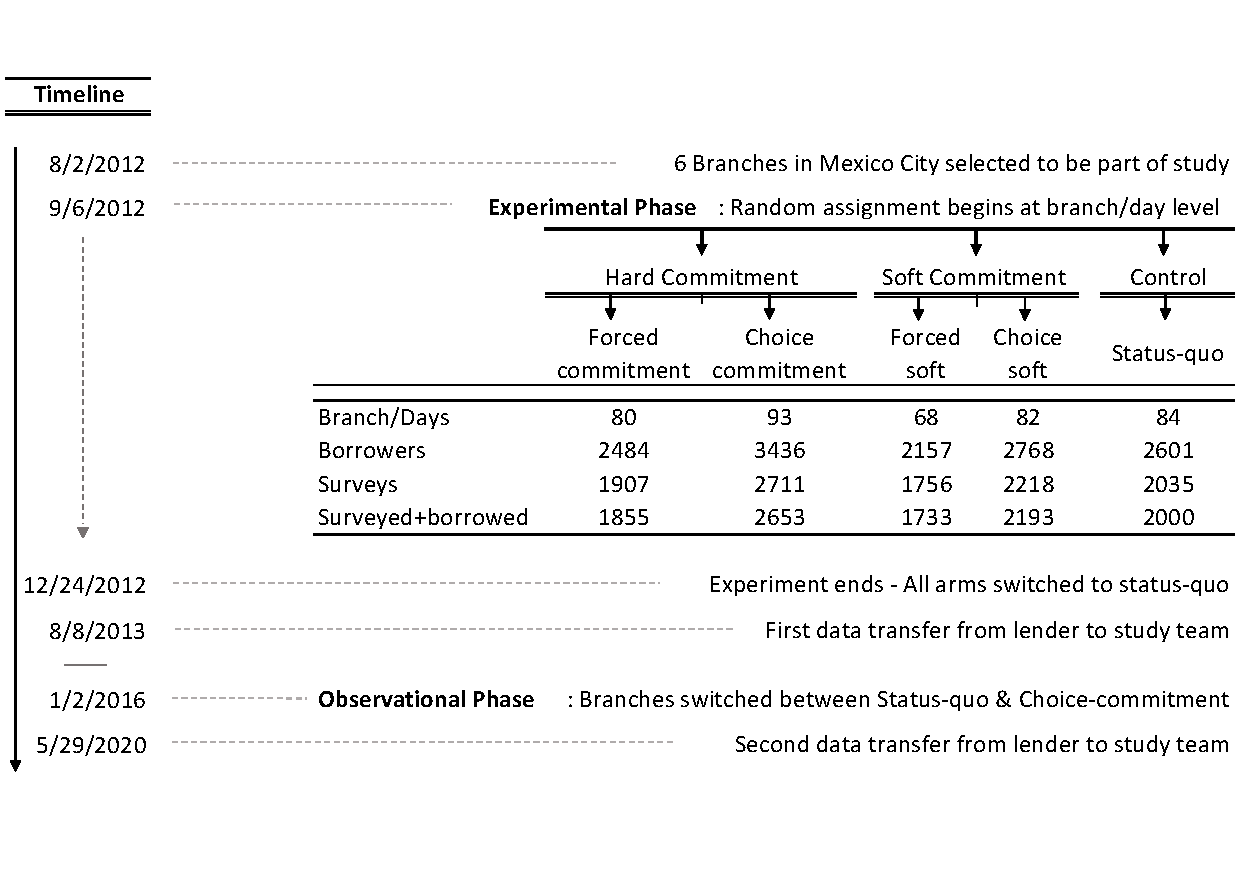
\includegraphics[width=0.85\textwidth]{Figuras/consort.pdf}
   \end{center}
 \end{figure}
 %\hyperlink{experimental_integrity}{\beamerbutton{Details}}
 \end{frame}


 

\begin{frame}{No differential selection}
\vspace{.2in}
    \begin{table}[H]
\label{attrition_table}
\begin{center}
\small{% Table generated by Excel2LaTeX from sheet 'Attrition'
\begin{tabular}{lcccr}
\toprule
      & Control & Structure & Choice & \multicolumn{1}{c}{p-value} \\
\midrule
\midrule
Loan take-up & 0.967 & 0.955 & 0.961 & 0.82 \\
      & (0.01) & (0.01) & (0.01) &  \\
\midrule
Number of borrowers & 20.8  & 22.2  & 25.4  & 0.17 \\
      & (3.29) & (3.9) & (4.89) &  \\
\rowcolor[rgb]{ .949,  .949,  .949} \multicolumn{1}{r}{median} & 19    & 20    & 21    & 0.5 \\
\midrule
Number of pawns/borrower & 1.4   & 1.4   & 1.4   & 0.43 \\
      & (0.08) & (0.04) & (0.05) &  \\
\rowcolor[rgb]{ .949,  .949,  .949} \multicolumn{1}{r}{median} & 1.4   & 1.3   & 1.3   & 0.6 \\
\midrule
Number of pawns  & 31    & 31.3  & 37.2  & 0.24 \\
      & (5.8) & (5.6) & (7.9) &  \\
\rowcolor[rgb]{ .949,  .949,  .949} \multicolumn{1}{r}{median} & 27    & 28    & 30    & 0.46 \\
\midrule
Amt borrowed/borrower & 2266.8 & 2094  & 2115.2 & 0.18 \\
      & (101.8) & (83.7) & (99.9) &  \\
\rowcolor[rgb]{ .949,  .949,  .949} \multicolumn{1}{r}{median} & 2154.3 & 2041  & 2047.5 & 0.65 \\
\midrule
Total borrowed & 47877 & 47813 & 54780 & 0.4 \\
      & (8005) & (9436) & (12587) &  \\
\rowcolor[rgb]{ .949,  .949,  .949} \multicolumn{1}{r}{median} & 37520 & 39420 & 40850 & 0.73 \\
\midrule
Obs   & 85    & 81    & 94    &  \\
\bottomrule
\bottomrule
\end{tabular}%
}
\end{center}
\end{table}
\end{frame}



\begin{frame}{Same characteristics across arms}
    \begin{table}[H]
\begin{center}
\resizebox{.55\textwidth}{!}{
\scriptsize{% Table generated by Excel2LaTeX from sheet 'SS'
\begin{tabular}{lcccccccc}
\toprule
      &       &       & \multicolumn{5}{c}{Treatment arms}    &  \\
\midrule
      &       &       &       & \multicolumn{2}{c}{No Choice } & \multicolumn{2}{c}{Choice} &  \\
\midrule
\midrule
      & Overall & Pre-experiment & Control & Fee   & Promise & Fee   & Promise & p-value \\
\midrule
      & \multicolumn{8}{c}{Panel A : Administrative Data} \\
\midrule
\midrule
Loan amount  & 2197  & 2239  & 2301  & 2147  & 2133  & 2181  & 2089  & 0.32 \\
      & (25)  & (39)  & (79)  & (72)  & (74)  & (65)  & (65)  &  \\
Monday & 0.18  & 0.16  & 0.18  & 0.16  & 0.17  & 0.19  & 0.21  & 0.96 \\
      & (0.02) & (0.03) & (0.05) & (0.05) & (0.06) & (0.06) & (0.05) &  \\
Number of branch-day pawns & 34    & 36    & 31    & 31    & 32    & 37    & 34    & 0.38 \\
      & (0.82) & (1.25) & (2.2) & (2.35) & (2.38) & (2.65) & (1.76) &  \\
\midrule
Number of branch-days & -     &       & 84    & 80    & 68    & 93    & 82    &  \\
Obs   & 21808 & 8366  & 2601  & 2484  & 2156  & 3435  & 2766  &  \\
\midrule
      & \multicolumn{8}{c}{Panel B : Survey Data (conditional on pawning)} \\
\midrule
\midrule
Woman & 0.73  &       & 0.76  & 0.72  & 0.73  & 0.72  & 0.74  & 0.41 \\
      & (0.01) &       & (0.02) & (0.02) & (0.02) & (0.02) & (0.01) &  \\
Age   & 43.31 &       & 43.16 & 43.17 & 42.96 & 43.96 & 43.06 & 0.79 \\
      & (0.28) &       & (0.57) & (0.79) & (0.65) & (0.61) & (0.52) &  \\
Subjective value & 3068  &       & 3151  & 2978  & 2985  & 3114  & 3079  & 0.41 \\
      & (39)  &       & (69)  & (91)  & (76)  & (85)  & (100) &  \\
Has pawn before & 0.9   &       & 0.89  & 0.9   & 0.89  & 0.91  & 0.89  & 0.68 \\
      & (0)   &       & (0.01) & (0.01) & (0.01) & (0.01) & (0.01) &  \\
Subj. pr. of recovery & 93.14 &       & 92.74 & 92.16 & 93.6  & 93.67 & 93.3  & 0.46 \\
      & (0)   &       & (0.55) & (0.86) & (0.6) & (0.47) & (0.6) &  \\
+High-school & 0.66  &       & 0.66  & 0.67  & 0.65  & 0.67  & 0.64  & 0.74 \\
      & (0.01) &       & (0.02) & (0.02) & (0.02) & (0.02) & (0.02) &  \\
Survey response rate & 0.78  &       & 0.77  & 0.75  & 0.8   & 0.77  & 0.79  & 0.5 \\
      & (0.01) &       & (0.02) & (0.03) & (0.02) & (0.02) & (0.02) &  \\
\midrule
Obs   & 10431 &       & 2000  & 1855  & 1732  & 2652  & 2192  &  \\
\midrule
\midrule
      & \multicolumn{8}{c}{Panel C : Survey Data (unconditional)} \\
\midrule
\midrule
Woman & 0.74  & 0.75  & 0.76  & 0.72  & 0.73  & 0.72  & 0.74  & 0.32 \\
      & (0.01) & (0.01) & (0.02) & (0.02) & (0.02) & (0.02) & (0.01) &  \\
Age   & 43.24 & 43.06 & 43.2  & 43.21 & 43.01 & 44.07 & 43.07 & 0.79 \\
      & (0.21) & (0.32) & (0.56) & (0.77) & (0.66) & (0.61) & (0.51) &  \\
Subjective value & 3112  & 3192  & 3145  & 2985  & 3010  & 3111  & 3082  & 0.41 \\
      & (36)  & (75)  & (68)  & (88)  & (76)  & (84)  & (99)  &  \\
Has pawn before & 0.89  & 0.88  & 0.89  & 0.9   & 0.89  & 0.91  & 0.89  & 0.56 \\
      & (0.01) & (0.01) & (0.01) & (0.01) & (0.01) & (0.01) & (0.01) &  \\
Subj. pr. of recovery & 92.64 & 91.84 & 92.73 & 92.19 & 93.66 & 93.71 & 93.34 & 0 \\
      & (0.2) & (0.31) & (0.54) & (0.84) & (0.59) & (0.46) & (0.59) &  \\
+High-school & 0.63  & 0.6   & 0.66  & 0.67  & 0.65  & 0.66  & 0.64  & 0.01 \\
      & (0.01) & (0.01) & (0.02) & (0.02) & (0.02) & (0.02) & (0.02) &  \\
\% ended up pawning &       &       & 0.98  & 0.97  & 0.99  & 0.98  & 0.99  & 0.25 \\
\midrule
Obs   & 17546 & 6919  & 2035  & 1907  & 1757  & 2710  & 2218  &  \\
\bottomrule
\bottomrule
\end{tabular}%
}
}
\end{center}
%\textit{Do file: } \texttt{ss\_att.do}
\end{table}
% \hyperlink{data}{\beamerbutton{Back}}
\end{frame}



\begin{frame}{Outline}
     \large   
     \begin{itemize}
        \item Context: Borrowers, contracts, data, outcomes
         \item \vfill ``Mandates-Choice'' Experimental Design
         \vfill\item \textbf{Main results}
          \vfill\item Exploiting ``Mandates-Choice'' Design: ToT, TuT
         \vfill\item Why low demand
         
     \end{itemize}
\end{frame}



%%%%%%%%%%%%%%%%%%%%%%%%%%%%%%%%%%%%%%%%%%%%%%%%
\section{Results}

\begin{frame}{Specification}
%\vspace{-1in}
\begin{equation} 
\Large
    y_{ij} = \alpha + \beta^S T_{i}^S + \beta^C T_{i}^C + \gamma X_{ij} + \epsilon_{ij}
\end{equation}

\begin{itemize}
    \vfill \item $i$-borrower, $j$-branch; $T_{i}^S$, $T_{i}^C$ indicator Structure or Choice arms; 
    \vfill\item Ommited category is the Status quo (pay-when-you-want).
    \vfill\item $X_{ij}$ branch + day-of-week fixed effects. Clustering branch-day level.
    \begin{itemize}
        \item 14\% pawned on two distinct days. We restrict our sample to each borrower's \emph{first visit}.
        \item A borrower (30\%) may pawn multiple items her visit. We include these as separate observations. Different contracts but the same contract type.
    \end{itemize}
    
    \vfill \item $\beta^C$ is the ATE of being given choice (or ITT of structure in the Choice arm).
    \vfill \item   $\beta^S$ is the ATE of mandatory structure (full compliance). 
\end{itemize}
\end{frame}


\begin{frame}{Large reductions in default and financial cost}
\label{main_results}
\begin{itemize}
    \item Financial cost reduced by \$204 pesos (22\% of mean). That is: charging fee + structure \textit{decreased} cost.
    \item Default decreases by 6.6pp (15\% of mean).
    \item APR decreases by 11$pp$, from mean of 57 percent yearly.
\end{itemize}
\vspace{.3in}
\begin{table}[H]
\begin{center}
\resizebox{0.95\textwidth}{!}{
\small{% Table generated by Excel2LaTeX from sheet 'decomposition_main_te'
\begin{tabular}{lcccccccc}
\cmidrule{3-7}      & FC    & Interest pymnt & Fee pymnt & Principal pymnt & Lost pawn value & Default &       & APR \\
\cmidrule{2-2}\cmidrule{9-9}      &       & $\sum_t P^i_{it}$ & $\sum_t P^f_{it}$ & $\mathds{1}(\text{Def}_i)}\times\sum_t P^c_{it}$ & $\mathds{1}(\text{Def}_i)}\times \text{Val-Loan Dif}_i$ & $\mathds{1}(\text{Def}_i)$ &       &  \\
\midrule
      & (1)   & (2)   & (3)   & (4)   & (5)   & (6)   &       & (7) \\
\midrule
\midrule
Forced commitment & -202.8*** & -157.3*** & 32.1*** & -0.61 & -77.6** & -0.065*** &       & -0.11*** \\
      & (48.1) & (34.9) & (1.43) & (2.88) & (31.6) & (0.023) &       & (0.019) \\
Choice commitment & -39.6 & -24.9 & 1.34** & -1.00 & -16.0 & -0.024 &       & -0.0089 \\
      & (49.8) & (38.4) & (0.54) & (2.62) & (33.1) & (0.021) &       & (0.019) \\
      &       &       &       &       &       &       &       &  \\
\midrule
Observations & 6304  & 6304  & 6304  & 6304  & 6304  & 6304  &       & 6304 \\
R-squared & 0.013 & 0.022 & 0.151 & 0.003 & 0.007 & 0.013 &       & 0.031 \\
Control Mean & 941.3 & 545.9 & 0     & 5.32  & 395.4 & 0.44  &       & 0.57 \\
\bottomrule
\bottomrule
\end{tabular}%
}
}
\end{center}
\end{table}
   \vfill 
  %\hyperlink{several_def_cost}{\beamerbutton{More}}
\end{frame}



\begin{frame}{Reduced costs even considering subjective value, travel, lost liquidity }

\vspace{-.1in}
\begin{itemize}
    \item Subjective value.
    \item Entire day's wage per visit + transport cost.
    \item Raw liquidity adjustment: as if she borrowed at 7\% to pay us.  %~(removed $\sum_t P^{I}_{it}$)
\end{itemize}
%\vspace{-.4in}
\begin{table}[H]
\label{table_robustness_fc}
\begin{center}
\resizebox{0.85\textwidth}{!}{
\small{\begin{tabular}{lccccc}
\toprule
      & FC    & FC (subj.value) & FC +  tc & FC + liq & FC (subj.value) + tc + liq \\
\midrule
      & (1)   & (2)   & (3)   & (4)   & (5) \\
\midrule
\midrule
Mandatory structured & -204.0*** & -299.9*** & -207.7*** & -98.5*** & -146.3** \\
      & (48.1) & (83.3) & (49.0) & (36.7) & (72.8) \\
Choice  & -38.9 & -56.4 & -32.6 & -30.7 & -25.3 \\
      & (49.8) & (83.5) & (50.9) & (39.2) & (74.4) \\
      &       &       &       &       &  \\
\midrule
Observations & 6304  & 6304  & 6304  & 6304  & 6304 \\
R-squared & 0.013 & 0.009 & 0.014 & 0.005 & 0.006 \\
Control Mean & 942.4 & 1389.9 & 1026.1 & 480.7 & 927.7 \\
\midrule
\midrule
\end{tabular}%}
}
\end{center}
 \scriptsize 
%\textit{Do file: } \texttt{fc\_robustness.do}
\end{table}
   % \hyperlink{main_results}{\beamerbutton{Back}}
\end{frame}


\begin{frame}{How savings come about: faster payments}
\begin{columns}
\begin{column}{.45\textwidth}
\begin{table}[H]
\begin{center}
\scriptsize{% Table generated by Excel2LaTeX from sheet 'mechanism_pres1'
\begin{tabular}{lcc}
\toprule
      & \multicolumn{2}{c}{Panel A  : Speed of payment} \\
\cmidrule{2-3}      & Days to 1st payment & \% of payment in 1st visit \\
\midrule
\midrule
      & (1)   & (2) \\
\midrule
\midrule
Forced cmit & -13.8*** & 7.69*** \\
      & (1.61) & (2.76) \\
Choice cmit & -3.51** & -1.11 \\
      & (1.57) & (2.19) \\
      &       &  \\
\midrule
Observations & 4412  & 6304 \\
R-squared & 0.055 & 0.014 \\
Control Mean & 82.8  & 44.8 \\
\midrule
\midrule
      &       &  \\
\midrule
      & $\Pr($Recovery in 1st visit) & \textcolor[rgb]{ .651,  .651,  .651}{Loan duration (days)} \\
\midrule
\midrule
      & (3)   & \textcolor[rgb]{ .651,  .651,  .651}{(4)} \\
\midrule
\midrule
Forced cmit & 0.079*** & \textcolor[rgb]{ .651,  .651,  .651}{-27.9***} \\
      & (0.026) & \textcolor[rgb]{ .651,  .651,  .651}{(4.35)} \\
Choice cmit & -0.010 & \textcolor[rgb]{ .651,  .651,  .651}{-0.18} \\
      & (0.022) & \textcolor[rgb]{ .651,  .651,  .651}{(4.33)} \\
      &       & \textcolor[rgb]{ .651,  .651,  .651}{} \\
\midrule
Observations & 6304  & \textcolor[rgb]{ .651,  .651,  .651}{6304} \\
R-squared & 0.016 & \textcolor[rgb]{ .651,  .651,  .651}{0.054} \\
Control Mean & 0.30  & \textcolor[rgb]{ .651,  .651,  .651}{136.6} \\
\bottomrule
\bottomrule
\end{tabular}%
}
\end{center}
\end{table}
\end{column}
\begin{column}{.45\textwidth}
   \begin{itemize}
     \item The first payment occurs 13 days earlier, and they pay 9\% more.
     \vspace{.2in}
     \vfill \item Increasing the fraction who recover on the first visit by 7.9 pp. 
     \vspace{.2in}
     \vfill  \item Loan resolution 28 days faster.
\end{itemize} 
\end{column}
\end{columns}
%\hyperlink{intermediate_outcomes}{\beamerbutton{Back}}
\end{frame}




\begin{frame}{Payment Bifurcation: less paying without recovering}
\begin{table}[H]
\begin{center}
\footnotesize{% Table generated by Excel2LaTeX from sheet 'mechanism_pres'
\begin{tabular}{lccc}
\toprule
      & \multicolumn{3}{c}{Panel B  : Variables related to default} \\
\cmidrule{2-4}      & $\Pr($+ payment \& default) & \% of pay $|$ def  & $\Pr($Selling pawn $|$ def) \\
\midrule
\midrule
      & (5)   & (6)   & (7) \\
\midrule
\midrule
Forced cmit & -0.071*** & -4.12*** & 0.14*** \\
      & (0.015) & (1.28) & (0.034) \\
Choice cmit & -0.027** & -1.82* & 0.050* \\
      & (0.014) & (1.05) & (0.029) \\
      &       &       &  \\
\midrule
Observations & 6304  & 2492  & 2492 \\
R-squared & 0.011 & 0.024 & 0.034 \\
Control Mean & 0.12  & 9.68  & 0.71 \\
\bottomrule
\bottomrule
\end{tabular}%
}
\end{center}
\end{table}

%\hyperlink{intermediate_outcomes}{\beamerbutton{Back}}
   \vfill \item   %Mandatory structure decreases fraction of borrowers making a payment and \textit{not} recovering by 7.1pp.
   As if Structure made them realize they will end up losing pawn anyway, and to stop paying early.
    % \begin{itemize}
    %     \item Among those that default, those in the forced commitment arm are 14pp less likely to have paid towards recovery. 
    % \end{itemize}
\end{frame}


% \begin{frame}{Visit Frequency}
%     \begin{table}[H]
% \begin{center}
% \footnotesize{% Table generated by Excel2LaTeX from sheet 'mechanism_pres'
\begin{tabular}{lcc}
\toprule
      & \multicolumn{2}{c}{Panel C  : Visit variables} \\
\cmidrule{2-3}      & \# of visits & \# of visits $|$ def \\
\midrule
\midrule
      & (8)   & (9) \\
\midrule
\midrule
Mandatory structured & 0.031 & -0.20*** \\
      & (0.049) & (0.050) \\
Choice  & 0.085 & 0.079* \\
      & (0.053) & (0.043) \\
      &       &  \\
\midrule
Observations & 6304  & 2492 \\
R-squared & 0.022 & 0.0028 \\
Control Mean & 1.14  & 0.39 \\
\bottomrule
\bottomrule
\end{tabular}%
}
% \end{center}
% \end{table}
% \vfill
% %\hyperlink{intermediate_outcomes}{\beamerbutton{Back}}
%  \begin{itemize}
%      \item \vfill Commitment induces a ``parting of the waters'' whereby those who were going to default visit the branch subsequently 1/5 fewer times.
% \end{itemize}
% \end{frame}





\begin{frame}{Do lenders profit from Structure?}

\begin{itemize}
    \item On a given pawn, borrowers gain = lenders loss.
    \item But, borrowers may return if they like the product. Do they? \pause Yes = 6.7pp higher repeat business. 
\end{itemize}
\begin{table}[H]
\begin{center}
\footnotesize{% Table generated by Excel2LaTeX from sheet 'repeat_loans'
\begin{tabular}{lcccHcc}
\toprule
      & \multicolumn{5}{c}{Ever pawns again (ITT)} \\
\cmidrule{2-6}      &       & After 90 days & Within 90 days & Different collateral & Cond. on rec \\
\midrule
\midrule
      & (1)   & (2)   & (3)   & (4)   & (4) \\
\midrule
\midrule
Mandatory structured & 0.067* & 0.037*** & 0.032 & 0.044 & 0.11** \\
      & (0.035) & (0.013) & (0.027) & (0.030) & (0.047) \\
Choice  & 0.040 & 0.0098 & 0.030 & 0.038 & 0.057 \\
      & (0.031) & (0.0087) & (0.026) & (0.028) & (0.042) \\
      &       &       &       &       &  \\
\midrule
Observations & 4441  & 4441  & 4441  & 4441  & 2170 \\
R-squared & 0.003 & 0.006 & 0.001 & 0.002 & 0.008 \\
Control Mean & 0.32  & 0.020 & 0.30  & 0.30  & 0.35 \\
\bottomrule
\bottomrule
\end{tabular}%}
\end{center}
\end{table}    
% \begin{itemize}
%     \item Client forced into commitment is 20\% more likely to come back again and pawn.
%     \item Not mechanically from having recovered the pawned, since also pawn other pieces.
%     \item Not within the life of the loan, but after. So unlikely that is a liquidity story.
%     \item Conditional on recovery (endogenous), ``effect'' twice as big.
% \end{itemize}
    
\end{frame}



\begin{frame}{Highly stylized Back-of-the-Envelope Profit }

\begin{itemize}
    \item Does repeat business compensate the loss per pawn? No, profit is at least 14\% \textit{lower} under structure.
    \vfill \item Calculate a discounted sum of profits for client $j$ comparing a scenario where (a) only status quo loans are offered with a second scenario where (b) only structured payment loans are offered.
    \vfill \item Let $\text{Profit}_{j,X}  = \sum_{t=0}^T\delta^t\{\text{Financial Cost}_j | \text{Contract}=X\}\times\Pr(\text{Repeat}_j | \text{Contract}=X)^t$, where $\delta$ is the discount rate, $X \in \{SQ, Structured\}$. 
    \begin{itemize}
        \item Going to the branch again assumed as independent events.
        \item We find that for every  $\delta$ $\in$ [0,1]  and for every $T$ the status quo results in at least 14\% higher profit for the lender.
    \end{itemize} 
    \vfill\item The extra repeat probability for the structured payment contract is insufficient to compensate for the loss in each loan.

    \vfill\item This may explain why lenders do not offer frequent payment contracts (in contrast with microfinance).
\end{itemize}
 
\end{frame}





\begin{frame}{Low demand for a feature that decreases financial cost?}
    \begin{itemize}
        \item Recap: structured payments save borrower's money, on average.
        \vfill \item  \textbf{However, only 11\% demand Structured payments contract}.
        \begin{itemize}
            \item More demand by: higher schooling, less experienced, less vulnerable, would like reminders.
        \end{itemize}
        \vfill\item Could it be that the 89\% \alert{who did not choose} would not benefit?
        \vfill\item Hard question, person level effects  $Y_{i1} - Y_{i0}$ are not identified.
        \begin{itemize}
            \item Non-parametric Fan and Park (2010) bounds imply \textcolor{green}{at least 23\% of borrowers would benefit}, so at least 12\% would have had lower FC and did not choose structure. 
        \end{itemize}
        \vfill\item Would like to know the avg. effect of non-choosers (\alert{Treatment on the Untreated}). 
    \end{itemize}
\end{frame}




\section{TuT vs ToT}

\begin{frame}{Outline}
     \large   
     \begin{itemize}
        \item Context: Borrowers, contracts, data, outcomes
         \item \vfill ``Mandates-Choice'' Experimental Design
         \vfill\item Main results
          \vfill\item \textbf{Exploiting ``Mandates-Choice'' Design: ToT, TuT, ASG}
         \vfill\item Why low demand
         
     \end{itemize}
\end{frame}




 
\begin{frame}{Identification afforded by experiment}
Our 3-arm experiment + exclusion restriction allows us to estimate: 
\begin {itemize}
 \item Treatment on the Treated (ToT).
 \item Treatment on the Untreated (TuT).
\end{itemize}
\vspace{.1in}
Notation: 
\begin{itemize}
    \item Potential outcomes $(Y_0,Y_1,C)$, where $C$ is borrower's ``choice-type'' $\in\{0,1\}$, i.e. $\{SQ,Structure\}$
    \item Assignment: $Z \in \{0,1,2\}$, i.e. $\{SQ,Structure,Choice\}$.  
    \item Treatment: $D \in \{0,1\} $, i.e. $\{SQ,Structure\}$.
\end{itemize}
\vspace{.1in}
Assumptions:
\begin{itemize}
     \item $Z \perp (Y_0,Y_1,C)$, achieved by randomization.
    \item $D = I(Z_i \neq 2) Z + I(Z_i=2) C$.
\end{itemize}
\end{frame}




\begin{frame}{ToT and TuT are identified}
Exclusion restrictions (for a given person $i$):
\begin{itemize}
        \item No agency effect 
        (NAE) from choosing: $Y_i(d=1,z=2)=Y_i(d=1,z=1) \equiv Y_{i1}$
        \item  No agency effect from not choosing: $Y_i(d=0,z=2)=Y_i(d=0,z=0) \equiv Y_{i0}$
    \end{itemize}
\pause \vfill This allows us to write the outcome for borrower $i$ as:
\begin{center}
    $Y_i = I(Z_i =0) Y_{i0} + I(Z_i = 1)  Y_{i1}  + I(Z_i = 2) \left[(1 - C_i) Y_{i0} + C_i Y_{i1} \right]$
\end{center}
   
\begin{itemize}
    \item Note $F_0$, $F_1$, and $C$ are identified.
\end{itemize}
\vspace{.1in}

\pause Prop:
\begin{itemize}
    \item ToT := $E(Y_{i1} - Y_{i0} | C_i = 1)$ is point-identified, and equals $\frac{E(Y_i|Z_i=2) - E(Y_i|Z_i =0)}{E(D_i|Z_i=2)} $
     \item TuT := $E(Y_{i1} - Y_{i0} | C_i = 0)$ is point-identified, and equals $\frac{E(Y_i|Z_i=1) - E(Y_i|Z_i =2)}{1-E(D_i|Z_i=2)} $
     %\item Also identified: 
     %\begin{itemize}
      %   \item Average Selection on Gains $ASG:=ToT-TuT$
         %\item Average Seletion Bias $ASB:= \E[Y_0 | C=1]-\E[Y_0 | C=0]$
         %\item Average Selection on Levels $ASL:= \E[Y_1 | C=1]-\E[Y_1 | C=0]$
     %\end{itemize}
\end{itemize}
\end{frame}





\begin{frame}{The ``Mandates-Choice'' Design}

\begin{itemize}
    \vfill \item Recall that under one-sided non-compliance (no always-takers), LATE=ToT.
    \vfill\item ToT: encouraged to choose Strucutre. 
 \vfill\item TuT: encouraged NOT to choose Structure. 
\end{itemize}
%\vspace{.2in}
\begin{figure}[H]
    \begin{center}
        \centering
        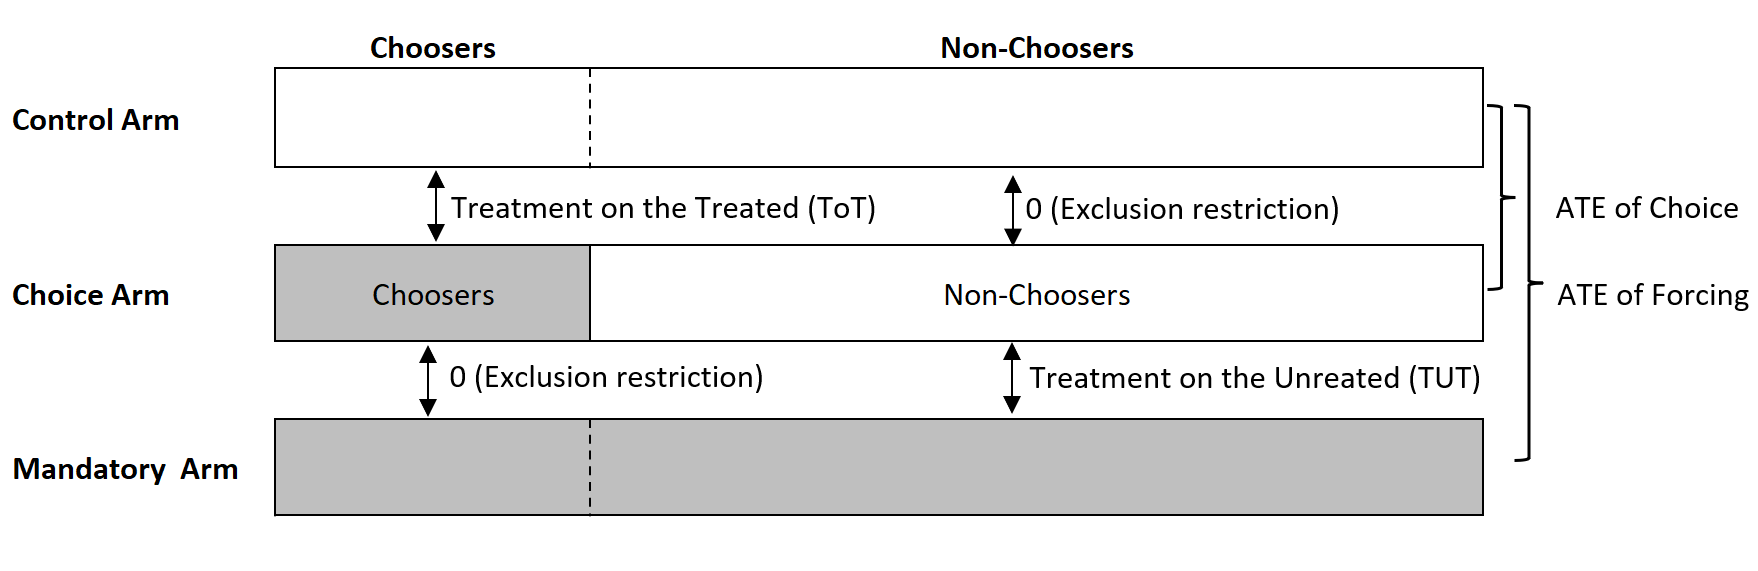
\includegraphics[width=.8\textwidth]{Figuras/tot_tut_graph.png}
    \end{center}
\end{figure}   
 \vfill
%\hyperlink{identification_randomized_choice}{\beamerbutton{Identification}}
\end{frame}




\begin{frame}{On avg. those that do \textit{not} choose would benefit: TuT $>$ 0}
\begin{itemize}
    \vfill \item Structure increases avg. financial benefit those who \alert{would not} choose it.
    \vfill \item  No selection on gains (ToT=TuT), in fact FC coefficients are smaller for ToT than for TuT.
    %\vfill \item Results hold when imputing transport cost and lost wages per visit, and charge interest in amount paid (as a proxy for liquidity lost).
\end{itemize}
\vspace{.1in}
\begin{table}[H]
%those who are most likely to benefit from it and those whose outcomes are most adverse under the status quo.
\label{tot_tut}
\begin{center}
\small{% Table generated by Excel2LaTeX from sheet 'tot_tut'
\begin{tabular}{lcccHc}
\toprule
      & APR \% benefit & FC benefit & \% (1-Default) & \% (1-Refinance) \\
\midrule
\midrule
ATE   & 9.41*** & 183.0*** & 7.74*** & 6.34** \\
      & (2.06) & (50.8) & (2.50) & (2.90) \\
ToT   & -0.59 & 111.9 & 37.4* & -25.9 \\
      & (21.4) & (528.3) & (21.6) & (29.1) \\
TuT   & 10.6*** & 191.5*** & 4.20* & 10.2*** \\
      & (2.47) & (50.8) & (2.41) & (2.90) \\
\midrule
ASG   & -11.2 & -79.6 & 33.2  & -36.1 \\
      & (22.9) & (556.2) & (22.6) & (30.6) \\
\midrule
Observations & 6304  & 6304  & 6304  & 6304 \\
%$H_0$ : ATE-TuT=0 & 0.62  & 0.89  & 0.14  & 0.23 \\
%$H_0$ : ATE-ToT=0 & 0.63  & 0.89  & 0.14  & 0.24 \\
$H_0$ : ASG=0 & 0.63  & 0.89  & 0.14  & 0.24 \\
%$H_0$ : ASG$\geq$ 0 & 0.69  & 0.56  & 0.071 & 0.88 \\
\bottomrule
\bottomrule
\end{tabular}%
}
\end{center}
\end{table}
\begin{center}
\vspace{-.1in}
\scriptsize{\centering Written now as a benefit ($\times$ -1). Numbers differ slightly as we don't include branch and day FE.}  
\end{center}
\end{frame}

% Despite substantial treatment effect heterogeneity, most borrowers would experience higher financial benefits under a commitment contract : $F_{\operatorname{TUT}}^{-1}(0.72)>0$




\begin{frame}{Recap}
We have learned that:
\begin{itemize}
     \item Forcing Structure ATE > 0 $\Rightarrow$ leads to positive financial benefit. 
    \pause \vfill \item   Choice ATE = 0 $\Rightarrow$  giving choice does \textit{not} increase financial benefit. 
    \pause \vfill \item A large part of this is due to low demand for structure.
    \pause \vfill\item TuT>0 $\Rightarrow$ argument for compulsory treatment \alert{(paternalism)}
\end{itemize}
    \pause  \vfill Three obvious questions (evidence is weaker but suggestive here):
    \begin{itemize}
        \item Why is demand ``low''?
        \item Would they learn over time that structure saves cost? 
        \item Can we target structure only to those that benefit instead of implementing a universal mandate?
    \end{itemize}
\end{frame}


\section{Why would there be low demand?}

\begin{frame}{Outline}
     \large   
     \begin{itemize}
        \item Context: Borrowers, contracts, data, outcomes
         \item \vfill ``Mandates-Choice'' Experimental Design
         \vfill\item Main results
          \vfill\item Exploiting ``Mandates-Choice'' Design: ToT, TuT
         \vfill\item \textbf{Why low demand:} suggestive evidence
         
     \end{itemize}
\end{frame}



\begin{frame}{If structure works, why don't people choose it?}
\begin{itemize}
    \item \textbf{1. Learning?} one possibility is that they would eventually demand it as they try it.
    \begin{itemize}
        \item One problem is that lenders may not provide it.
        \item (Experience pawning \textit{negatively} correlated with take up of structure).
    \end{itemize}
    \vfill \item  Test those assigned to Structure or Status quo return and have a choice (i.e. get choice arm).
        \begin{itemize}
        \item Problems: small sample and returning is endogenous.
    \end{itemize}
 \end{itemize}  
 \vspace{.1in}
\begin{table}[H]
\begin{center}
 \resizebox{0.65\textwidth}{!}{
\small{% Table generated by Excel2LaTeX from sheet 'learning_exp'
\begin{tabular}{lccc|ccc}
\toprule
      & \multicolumn{3}{c|}{Choose Fee} & \multicolumn{3}{c}{Choose Promise} \\
\midrule
      & (1)   & (2)   & (3)   & (4)   & (5)   & (6) \\
\midrule
\midrule
Fee-forcing (FF) & 0.078 & 0.016 & 0.090 & 0.094 & -0.029 & 0.17 \\
      & (0.076) & (0.087) & (0.12) & (0.11) & (0.15) & (0.16) \\
Fee-promise (FP) & 0.085 & 0.033 & 0.19  & -0.030 & -0.082 & -0.14 \\
      & (0.11) & (0.034) & (0.17) & (0.18) & (0.28) & (0.20) \\
Choice/SQ (CSQ) & 0.069 & 0.10  & 0.14  & 0.085 & 0.12  & 0.17 \\
      & (0.063) & (0.063) & (0.13) & (0.071) & (0.11) & (0.11) \\
Choice/Fee (CF) & -0.049 & -0.094 & -0.017 & -0.20 & 0.26  & -0.28 \\
      & (0.10) & (0.10) & (0.14) & (0.16) & (0.29) & (0.22) \\
Decision epoch 2 (D2) &       & -0.16 &       &       & -0.21 &  \\
      &       & (0.16) &       &       & (0.22) &  \\
Decision epoch 3 D(3) &       & 0.037 &       &       & 0.027 &  \\
      &       & (0.034) &       &       & (0.15) &  \\
FF\#D2 &       & 0.17  &       &       & 0.46  &  \\
      &       & (0.20) &       &       & (0.28) &  \\
FF\#D3 &       & -0.017 &       &       & -0.14 &  \\
      &       & (0.081) &       &       & (0.27) &  \\
FP\#D2 &       & 0.49  &       &       & 0.30  &  \\
      &       & (0.29) &       &       & (0.34) &  \\
FP\#D3 &       & -0.30 &       &       & -0.016 &  \\
      &       & (0.27) &       &       & (0.39) &  \\
CSQ\#D2 &       & 0.096 &       &       & 0.12  &  \\
      &       & (0.16) &       &       & (0.24) &  \\
CSQ\#D3 &       & -0.16 &       &       & -0.044 &  \\
      &       & (0.084) &       &       & (0.18) &  \\
CF\#D2 &       & 0.062 &       &       & -0.38 &  \\
      &       & (0.29) &       &       & (0.29) &  \\
CF\#D3 &       & 0.071 &       &       & -0.39 &  \\
      &       & (0.16) &       &       & (0.36) &  \\
Default (Def) &       &       & 0.15  &       &       & 0.12 \\
      &       &       & (0.13) &       &       & (0.14) \\
FF\#Def &       &       & 0.19  &       &       & -0.17 \\
      &       &       & (0.25) &       &       & (0.20) \\
FP\#Def &       &       & -0.23 &       &       & 0.13 \\
      &       &       & (0.18) &       &       & (0.24) \\
CSQ\#Def &       &       & -0.13 &       &       & -0.17 \\
      &       &       & (0.13) &       &       & (0.17) \\
CF\#Def &       &       & 0.031 &       &       & 0.11 \\
      &       &       & (0.14) &       &       & (0.30) \\
      &       &       &       &       &       &  \\
\midrule
Observations & 150   & 150   & 150   & 152   & 152   & 152 \\
R-sq  & 0.720 & 0.768 & 0.763 & 0.640 & 0.681 & 0.651 \\
DepVarMean & \multicolumn{3}{c|}{0.053} & \multicolumn{3}{c}{0.20} \\
Individual FE & \checkmark & \checkmark & \checkmark & \checkmark & \checkmark & \checkmark \\
\bottomrule
\bottomrule
\end{tabular}%
}
}
\end{center}
\end{table}
 %\hyperlink{learning}{\beamerbutton{Back}}
\end{frame}



\begin{frame}{Can impatience explain it?}
    \begin{itemize}
    \item  Structured payments imposes up-front costs for later benefits (collateral recovery).  
    \item  Requires annual discounting > 4,000\% to make NPV TuT =0. 
    \end{itemize}
\vspace{.1in}
\begin{figure}[H]
    \begin{center}
        \centering
        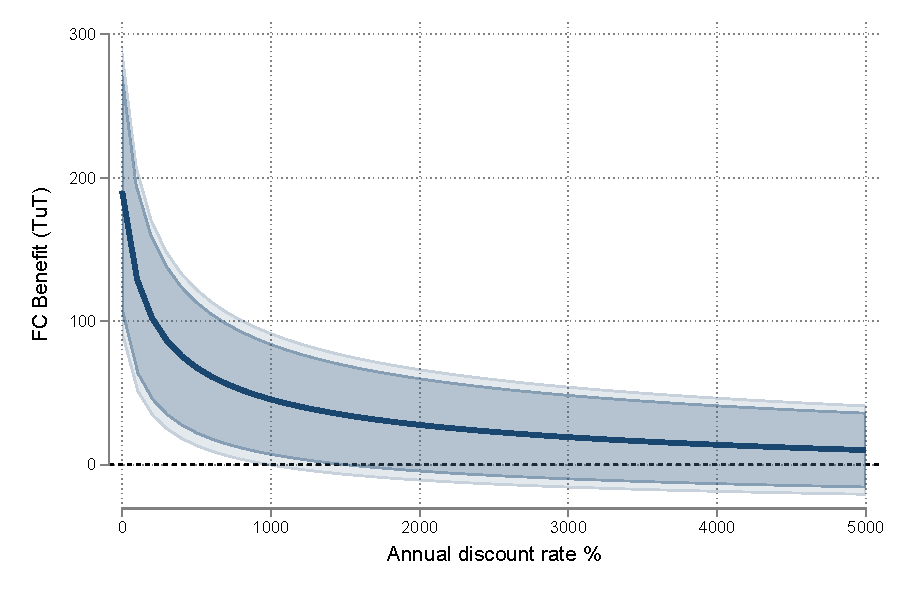
\includegraphics[width=0.50\textwidth]{Figuras/discount_effect_tut.pdf}
    \end{center}
\end{figure}   
\end{frame}



\begin{frame}{Time inconsistency? (very stylized)}

 \textbf{Canonical behavioral angle: Present bias}  PB naifs may not demand structure, yet have TuT>0

\begin{figure}[H]
    \begin{center}
        \centering
        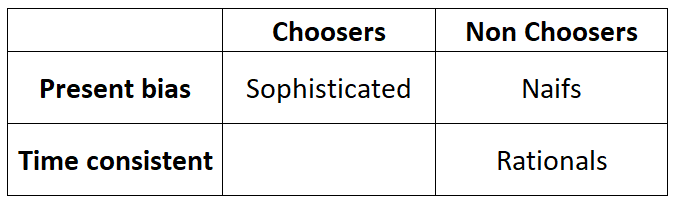
\includegraphics[width=0.4\textwidth]{Figuras/hyperbolicity_strata.png}
    \end{center}
\end{figure}   
    \pause \begin{itemize}
    \item Survey ``switching'' measure of time inconsistency. %(\$100 tomorrow or \$150 in one month; and then 3 vs 4 months).
    \begin{itemize}
        \item Also questions about them falling into spending ``temptation'', and wanting reminders.
    \end{itemize}
     
    \vfill \item  Prediction: because Structure should not help rationals, TuT should be positive only among the PB-non choosers (=naifs).   
    \item We don't find this,  but the PB measure may not be good.
    
    \end{itemize}
\end{frame}




\begin{frame}{Overconfidence?}

\begin{itemize}
    \item   Recall that at baseline, people were, on average, overconfident about recovering pawns.
    \vfill \item We find that TuT>0 is concentrated on those (28\%) that said they will recover with 100\% probability. 
    \begin{itemize}
        \item Conceptually, overconfidence could explain low take up and TuT>0.
        \item Intuitively: overconfidents underappreciate the benefit of structure.
    \end{itemize}
    %\vfill \item In contrast, we don't find this result for PB (as measured by us).
\end{itemize}
\begin{figure}[H]
        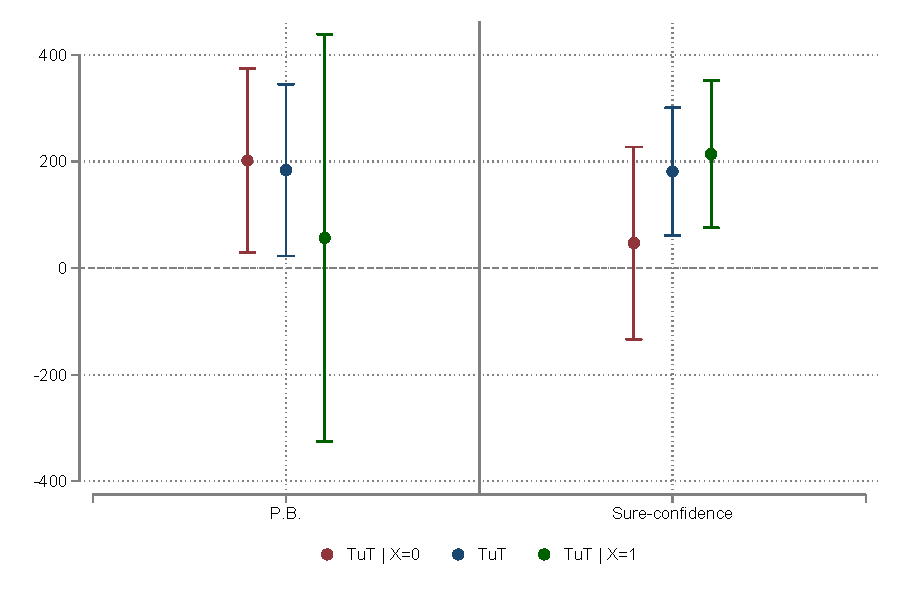
\includegraphics[width=0.5\textwidth]{Figuras/tut_beh_partition.pdf}
\end{figure}
\end{frame}



\begin{frame}{Sure confidence and Present bias}
        % \begin{figure}
        % \caption{What attributes correlate with Sure Confidence?}
        % \centering
        % 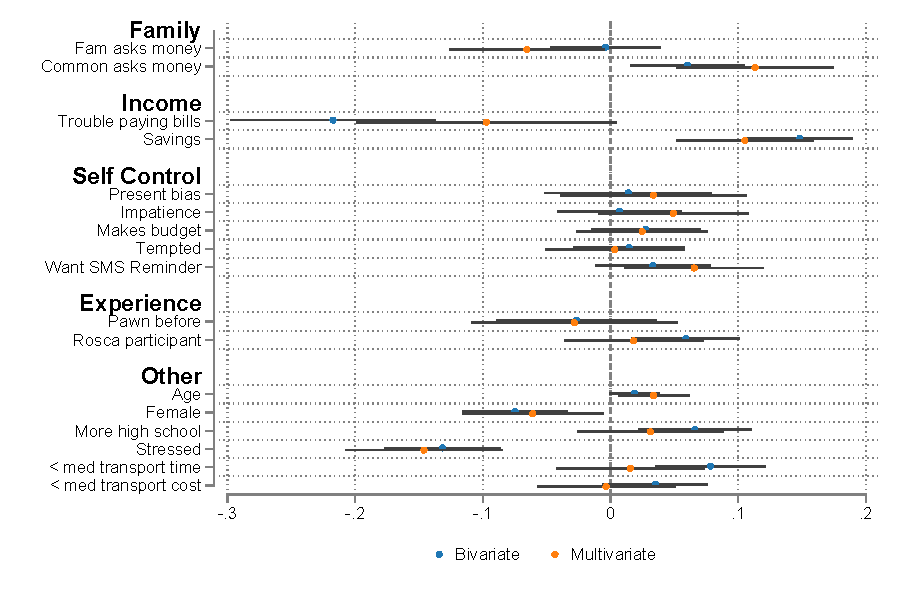
\includegraphics[width=0.65\textwidth]{Figuras/determinants_confidence_100.pdf}
        % \end{figure}
Do we need to model overconfidence and PB?
\begin{itemize}
    \item We can think of borrower overconfidence of recovery arising from a belief that their distribution of future income is shifted to the right vis-a-vis the real one.
    \item It can also come from PB naivete itself, as those types will spend more than expected and have less money to pay.
\end{itemize}
\vfill Determinants of Sure Confidence. The Sure-Confident are:
\begin{itemize}
    \item   Older, more educated men who
    \item   Have savings and do not report financial stress or trouble meeting bills, and 
    \item   Are likely to be relied upon by family members.
\end{itemize}   

\end{frame}



\begin{comment}
    
\begin{frame}{Do we need to model overconfidence and PB? (sketch)}

\begin{itemize}
    \item We can think of borrower overconfidence of recovery arising from a belief that their distribution of future income is shifted to the right vis-a-vis the real one.
    \begin{itemize}
        \item It can also come from PB naivete itself, as those types will spend more than expected and have less money to pay.
    \end{itemize}
   \pause \vfill  \item Simple model features PB and overconfidence, 3 periods: 
\begin{itemize}
        \item Period 3 (default): Pay iff: $u\bigl(y_3 - R \cdot \mathit{\text{Outstanding  debt}}\bigr) + v 
\;>\; u(y_3)$.   
  \item Period 2: Pay interim $\kappa$ iff \[
u(y_2 - k)
\;+\;
\beta\,\delta 
\;\mathbb{E}_{y_3|y_2,y_1}\Bigl[\max\bigl\{\,u\bigl(y_3 - R(L - k)\bigr) + v,\;u(y_3)\bigr\}\Bigr]
\quad\]
\[>\quad
u(y_2)
\;+\;
\beta\,\delta
\;\mathbb{E}_{y_3|y_2,y_1}\Bigl[\max\bigl\{\,u\bigl(y_3 - R\,L\bigr) + v,\;u(y_3)\bigr\}\Bigr].
\]
        %\item Period 2: Get stochastic income $y_2$. In Structure contract pay $\kappa$; no payment required in SQ contract.
        \item Period 1: Decide on contract $\in$ \{SQ,Structure\} to Max discounted expected utility. 
    \end{itemize}
    \vfill\item We plan to have income follow a distribution $f(y;\mu)$, and overconfidents think $\hat{\mu}>\mu$. Model PB in the standard ($\beta,\delta$) way. 
    \pause \vfill\item Parameters: [L,R,$\kappa$,\delta$,$\beta$,$\hat{\beta},$\nu$,$\mu$]; Decisions: [$t_1$:(SQ or S), $t_2$:(pay $\kappa$ or not), $t_3$:(default and lose $\nu$)].
    \vfill\item Show that both PB naivete and OC can explain TUT>0 in the model.
\end{itemize}

\end{frame}

\end{comment}


\begin{comment}
    
% =======================
% Period T=3: Default vs. Repay
% =======================
\subsection{Period 3}
\[
\text{Repay if and only if}\quad
u\bigl(y_3 - R \cdot \mathit{\text{Outstanding  debt}}\bigr) + v 
\;>\;
u(y_3).
\]
\[
\text{Otherwise, default.}
\]
\[\text{Outstanding debt} =\begin{cases}
  L-k &\text{if pay in T=2}\\
  L &\text{if not pay in T=2}
\end{cases}\]

% =======================
% Period T=2: Pay k vs. Not Pay k
% =======================
\subsection{Period 2}
\[
u(y_2 - k)
\;+\;
\beta\,\delta 
\;\mathbb{E}_{y_3|y_2,y_1}\Bigl[\max\bigl\{\,u\bigl(y_3 - R(L - k)\bigr) + v,\;u(y_3)\bigr\}\Bigr]
\quad\]
\[>\quad
u(y_2)
\;+\;
\beta\,\delta
\;\mathbb{E}_{y_3|y_2,y_1}\Bigl[\max\bigl\{\,u\bigl(y_3 - R\,L\bigr) + v,\;u(y_3)\bigr\}\Bigr].
\]
\[
\text{If the left side is greater, pay } k; \text{ otherwise, do not pay } k.
\]
\vspace{5mm}

For overconfident people:
\[
u(y_2 - k)
\;+\;
\beta\,\delta 
\;\mathbb{E}_{y_3'|y_2,y_1}\Bigl[\max\bigl\{\,u\bigl(y_3 - R(L - k)\bigr) + v,\;u(y_3)\bigr\}\Bigr]
\quad>\quad
u(y_2)
\;+\;
\beta\,\delta
\;\mathbb{E}_{y_3'|y_2,y_1}\Bigl[\max\bigl\{\,u\bigl(y_3 - R\,L\bigr) + v,\;u(y_3)\bigr\}\Bigr].
\]

% =======================
% Period T=1: Commitment vs. No Commitment
% =======================
\subsection{Period 1}
\[
\underbrace{
\beta\,\delta\,\mathbb{E}_{y_2|y_1}[\,u(y_2)\,] 
\;+\;
\beta\,\delta^2
\,\mathbb{E}_{y_3|y_1}\Bigl[\max\bigl\{\,u\bigl(y_3 - R\,L\bigr)+v,\;u(y_3)\bigr\}\Bigr]
}_{\text{No-Prepayment}}
\quad\]

\[<\quad
\underbrace{
\beta\,\delta\,\mathbb{E}_{y_2|y_1}[\,u(y_2 - k)\,]
\;+\;
\beta\,\delta^2
\,\mathbb{E}_{y_3|y_1}\Bigl[\max\bigl\{\,u\bigl(y_3 - R(L-k)\bigr)+v,\;u(y_3)\bigr\}\Bigr]
}_{\text{Prepayment}}.
\]
\[
\text{Choose commitment if the right side is greater.}
\]
\end{comment}





\begin{frame}{Outline}
     \large   
     \begin{itemize}
        \item Context: Borrowers, contract, data, measures
         \item \vfill ``Mandates-Choice'' Experimental Design
         \vfill\item Main results
          \vfill\item Exploiting ``Mandates-Choice'' Design: ToT, TuT
         \vfill\item Why low demand
         \vfill \item \textbf{TE heterogeneity and targeting?}
     \end{itemize}
\end{frame}



\begin{frame}{TE heterogeneity in TuT}

\begin{columns}
\begin{column}{.43\textwidth}
\begin{figure}    
\centering
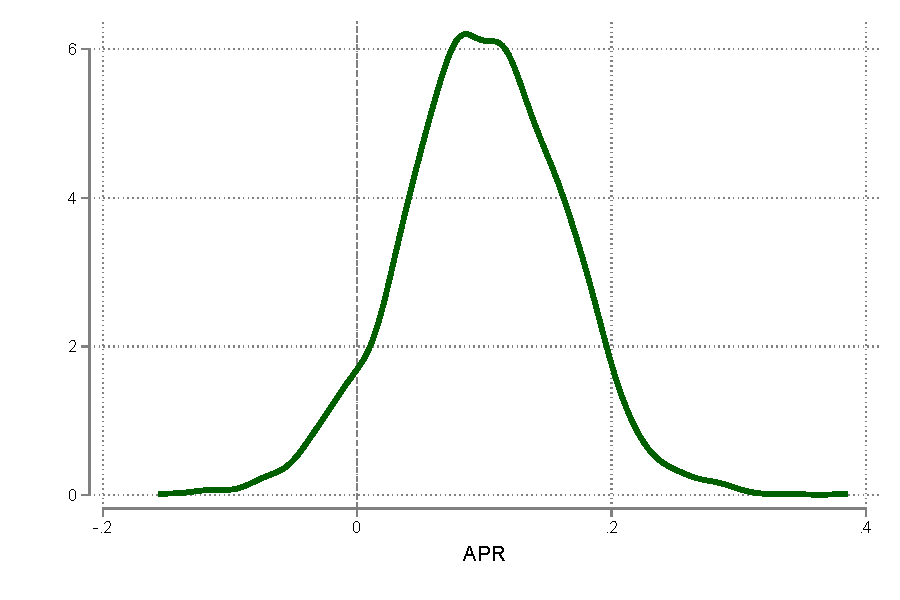
\includegraphics[width=0.99\textwidth]{Figuras/he_dist_tau_hat_tut.pdf}
\end{figure}
\end{column}
\begin{column}{.5\textwidth}
   \begin{itemize}
     \item Assuming NAE conditional on X's, we use (Athey et.al. 2019) causal forests to estimate $E[Y_1 - Y_0| X = \mathbf{x}, C = 0]$, i.e. CTuT
     \vspace{.1in}
     \begin{itemize}
	 \item Causal forest partition X to produce the biggest difference in TE across leaves, and gives a ``personalized'' TE according to the leaf borrowers are assigned to.
    \end{itemize}
    \vspace{.2in}
    \item Only 7\% of borrowers's estimated CTuT < 0.
    \vspace{.2in}
    \item >1/2 lose at least 10pp APR from not choosing.
    \end{itemize}
\end{column}
\end{columns}
\end{frame}



\begin{frame}{How well can we target Structure}
\begin{itemize}
    \item   Can we predict who would lose from structure, to assign them to status quo?
        %\vfill \item   Standard targeting analysis, except need to consider covariates carefully given context.
    %\vfill \item   Private sector lender, competitive market, part of attraction of pawning is no application!  
    \vfill \item Take (wide) Causal RF estimate $(Y_{i1}-Y_{i0})^{wide}$ (CATE) as ground truth.
    \vfill \item Use ``narrow'' causal RF (verifiable: age, gender, schooling, pawned before) as a targeting model,  
     \begin{itemize}
         \item Assign based on estimated $(Y_{i1}-Y_{i0})^{narrow}$.
         \item Define assignment of borrower $i$ to Structure as error if : $(Y_{i1}-Y_{i0})^{wide}<0$, and analogously for status quo.
     \end{itemize}

    \vfill \item Finding: our best targeting has 9\% ``errors'', as large as assigning \textit{everyone} to Structure. 
    %\item   Cannot use choice and then compel compliance among non-choosers in a commercial context.  
    \vfill\item Observed Choice has 87\% errors. 
    \vfill\item Given low take up + large fraction benefits from Structure (CATE) + benefit hard to predict with narrow variables $\rightarrow$ paternalistic mandate may be attractive.
    % \vfill \item Which leaves us with:
    % \begin{itemize}
    % \item   Age
    % \item   Gender
    % \item   HS Education or above
    % \item   Ever pawned before 
    % \end{itemize}
\end{itemize}        
\end{frame}



% \begin{frame}{Predicted APR CATEs `Wide' and `Narrow' }

%         \begin{figure}
%         %\caption{Scatterplot of Predicted Heterogeneity}
%         \centering
%         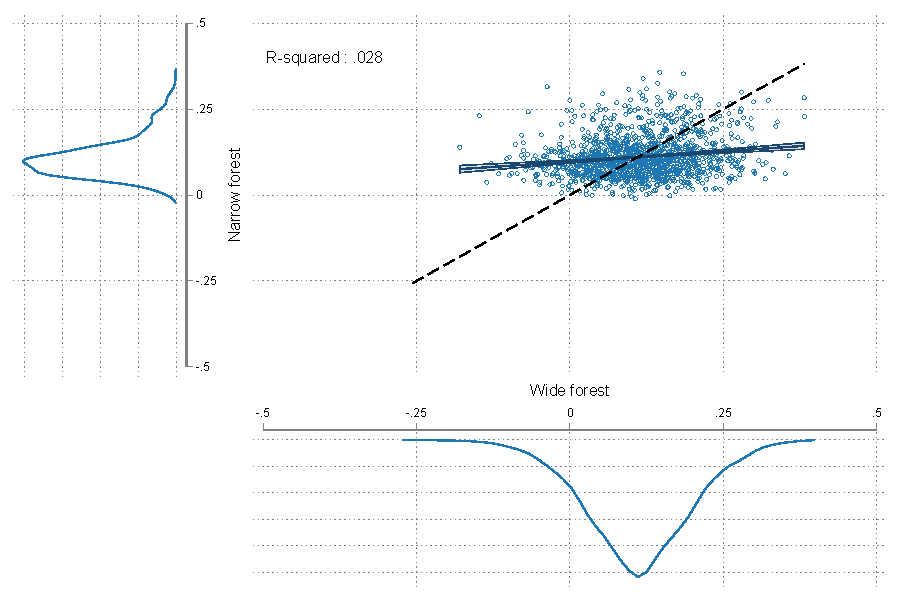
\includegraphics[width=0.6\textwidth]{Figuras/scatter_hist_wide_narrow.pdf}
%         \end{figure}

%\begin{itemize}
   % \item   Substantially less heterogeneity fitting APR CATE with `narrow' than `wide'
    %\item Test of homogeneity (Chernozhukov et. al. 2018) no longer rejected with `narrow'
    %\item   However, overall fitted relationship shows `narrow' adjusts to the mean TE.
%\end{itemize}        
%\end{frame}


%\begin{frame}{Comparison of Targeting Performance:  CDFs} 
%         \begin{figure}
%         \label{targeting_CDFs}
%         \caption{Distribution of Benefits under Different Targeting Rules}
%         \centering
%         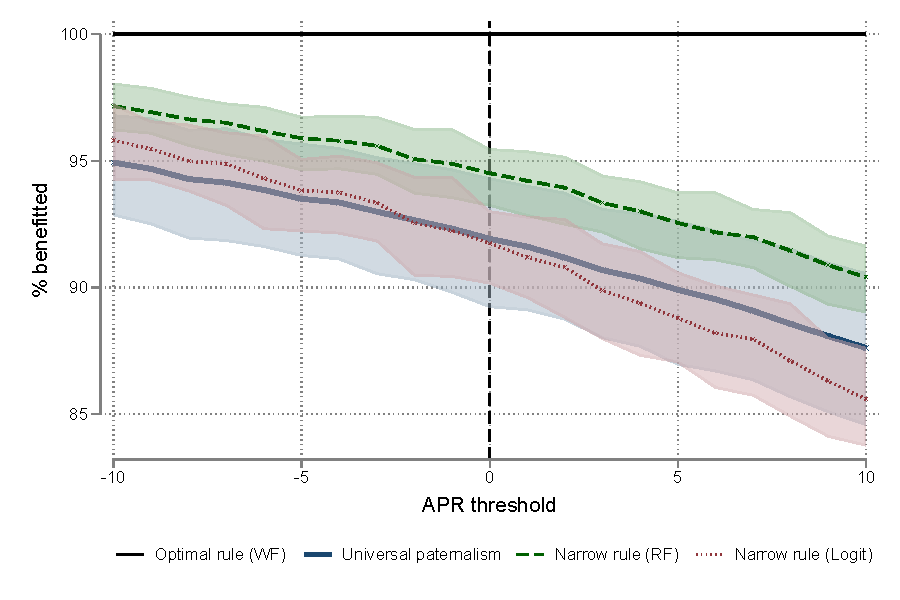
\includegraphics[width=0.70\textwidth]{Figuras/wide_narrow_rule.pdf}
%         \end{figure}
% \begin{itemize}
%     \item   Even using the Random Forest to target, our four `narrow' variables only increase the fraction benefitting from 91\% (all Forced) to ~93\% (targeted).
%     \item  Using a Logit with the `narrow' variables actually worsens performance relative to universal Forcing because Logit matches benefit/loss fraction, has both Type 1 and Type 2 errors.
% \end{itemize}        
% \end{frame}



% \begin{frame}{Type I \& II errors using targeting narrow rules}
% \begin{itemize}
%     \item Taking wide RF as the ground truth, compare Mandates vs choice, vs narrow targeting.
% \end{itemize}
% \vspace{.2in}
% \begin{table}[H]
% \begin{center}
% \resizebox{0.35\textwidth}{!}{
% \small{% Table generated by Excel2LaTeX from sheet 'hit_miss_rule2'
\begin{tabular}{lc}
\toprule
\multicolumn{1}{c}{Rule} & Overall Error Rate \\
      &  \\
\midrule
\midrule
All to status-quo & 90.22 \\
All to Structure & 9.78 \\
Allow choice & 87.4 \\
%Optimal  & 0 \\
Narrow rule (RF) & 9.59 \\
%Narrow rule (Logit) & 14.66 \\
\bottomrule
\bottomrule
\end{tabular}%
}
% }
% \end{center}
% \end{table} 
% \begin{itemize}
%     %\item   Even RF with `narrow' variables results in very modest increase in targeting efficiency relative to universal paternalism.
%     %\item  Logit performs very poorly because it makes symmetric Type I and Type II errors and hence assigns many to control who would have been better off with commitment.
%     \item  \textbf{Takeaway:}  With these variables, targeting mandated structure is ineffective; universal mandate achieves same outcome.
% \end{itemize}        
% \end{frame}



\section{Conclusion}
\begin{frame}{Conclusion}
    \begin{itemize}
     \item This paper analyzes the important but understudied industry of pawn loans, where over-collateralization and overconfidence may create a role for regulation.
     \vfill \item Simple change to contract terms results in substantial financial savings: mandatory structure lowers the APR from 57\% to 46\%, and reduces the fraction of borrowers who default by 6.6 pp.
    \vfill \item Novel RCT design to study take up and treatment heterogeneity (ToT, TuT, ASG): TuT>0, and no ASG. 
     \vfill \item Laibson has spoken of `\textit{private paternalism}', where firms supply commitment not demanded by consumers to the benefit of both. Pawn loans may be a contrary case, with lenders embedding features that \textit{hurt} borrowers.
     \vfill \item Q: (i) Would results hold using more comprehensive welfare measures? (ii) How would stronger lender competition affect the incentives to provide structured payment contracts? (iii) Would borrowers learn the benefits of structured payments in the longer run? 
    \end{itemize}  
\end{frame}


\begin{frame}{Contributions to Literature}

\begin{itemize}
    \item  Few studies of pawn lending.
    \vfill \item Mandates-vs-choice Design is new to the literature. Simultaneously identify both TOT, TUT, ASG without the need for auxiliary structural modeling assumptions. Fowlie et al (2021), Karlan and Zinman (2009), Beaman et al (2023) do not identify TUT effects. 
    \vfill \item Relatively small literature selection-on-gains and paternalism (e.g. Laibson 2018). Walters (2018): distance-based instrument with structural model, finds students who select into more effective schools have smaller treatment effects. Saddoff et al (2019) shows that individuals with the most time-inconsistent preferences in food choice are the least likely to demand commitment. 
    \vfill \item Contract design: Pande and Field (2008) find no effects from frequent repayment schemes. Field et al (2013), Barboni et al (2023) find productive benefit of flexibility in microfinance.
    \vfill \item Large literature on demand for commitment.  We separately point-identify and estimate the effects of commitment for borrowers who would and would not choose it. 
\end{itemize}
    
\end{frame}



\end{document}